% ============================================================
% main.tex
% Rapport de Master Mécanique
% Compilation : xelatex -> biber -> xelatex -> xelatex
% Nécessite : MemoireMaster.cls, references.bib
% ============================================================
%
% Directives de compilation :
% !TEX program = xelatex
% !BIB program = biber
% ============================================================

\documentclass[french]{MemoireMaster}

% ------------------------------------------------------------
% Police Garamond
% ------------------------------------------------------------
\IfFileExists{ebgaramond.sty}{%
  \usepackage{ebgaramond}
}{}

\usepackage{booktabs}
\usepackage{tabularx}
\usepackage{float}
\usepackage[style=numeric, backend=biber, sorting=none]{biblatex}
\defbibheading{bibliographie}{\section*{Références bibliographiques}}
\sisetup{
  locale = FR,
  detect-all
}

% ============================================================
% MÉTADONNÉES
% ============================================================

\titre{Modélisation des phénomènes de ségrégation granulaire à l'aide des chaînes de Markov inhomogènes}

\auteur{TONGUE Kevin}

\ecole{Centrale Lyon ENISE, Centrale Lyon, Université de Lyon}

\formation{Ingénieur génie Mécanique}

\entreprise{Georges Friedel (EMSE) --- RAPSODEE (IMT Mines Albi)}

\tuteurLabo{Guillaume Dumazer, Éric Serris (EMSE) ; Cendrine Gatumel (RAPSODEE)}

\tuteurEco{Éric Feulvarch (ENISE)}

\renewcommand{\dateDebut}{09/03/2026}
\renewcommand{\dateFin}{17/09/2026}
\dateSoutenance{02/09/2026}

% ============================================================
% PAGE DE GARDE
% ============================================================

\renewcommand{\parcoursMaster}{MNS}
\renewcommand{\laboratoireStage}{Georges Friedel (EMSE)}
\renewcommand{\adresseLaboratoire}{158 cours Fauriel, CS 62362, 42023 Saint-Étienne Cedex 2}
\renewcommand{\entrepriseStage}{RAPSODEE (IMT Mines Albi)}
\renewcommand{\adresseEntreprise}{Campus Jarlard, 81013 Albi Cedex 9}
\renewcommand{\encadrantLaboEntreprise}{%
  Guillaume Dumazer (EMSE)\\
  Éric Serris (EMSE)\\
  Cendrine Gatumel (RAPSODEE, Mines Albi)
}
\renewcommand{\encadrantEcole}{Éric Feulvarch }
\renewcommand{\juryPresident}{M./Mme ---}
\renewcommand{\juryMembreUn}{M./Mme ---}
\renewcommand{\juryMembreDeux}{M./Mme ---}

% ============================================================
% BIBLIOGRAPHIE
% ============================================================

\addbibresource{references.bib}

% ============================================================
% DOCUMENT
% ============================================================

\begin{document}

\pagestyle{empty}

\fairepagedegarde

% ============================================================
% REMERCIEMENTS
% ============================================================
\fairemerciements{%
  \noindent
  Je tiens tout d'abord à remercier mes encadrants de stage,  pour leur accompagnement rigoureux, leurs conseils avisés et leur disponibilité constante tout au long de ces six mois.
  Guillaume Dumazer pour sa vision et son interpretation de la physique du phénomène; Éric Serris pour ses conseils sur la construction des modèles,et des possibles applications . Cendrine Gatumel pour ses remarques les plus intéressantes
  qui ont permis de raisonner toujours plus dans un contexte industriel évitant une décorrelation entre le numérique et l'expérimental.

  % \vspace{0.4cm}
  % \noindent
  % Je remercie également mon encadrant école, Éric Feulvarch, pour son suivi attentif et ses orientations scientifiques qui ont nourri ma réflexion.

  \vspace{0.4cm}
  \noindent
  Mes remerciements s'adressent aux membres du jury pour l'évaluation de ce mémoire, ainsi qu'à l'ensemble des enseignants de l'ENISE pour la qualité de la formation dispensée.

  % \vspace{0.4cm
  % \noindent
  % Enfin, je remercie chaleureusement les membres du laboratoire Georges Friedel et du centre RAPSODEE pour leur accueil bienveillant et les échanges scientifiques stimulants qui ont rythmé cette période.
}
% ============================================================
% RÉSUMÉ FRANÇAIS
% ============================================================
\section*{Résumé}

\noindent
Omniprésents dans l'industrie --- agroalimentaire, pharmacie, nucléaire, construction ---, les milieux granulaires posent un défi majeur : maîtriser leur mélange et anticiper leur ségrégation. Ce mémoire développe une approche stochastique fondée sur les chaînes de Markov pour reproduire la dynamique de particules bidisperses (\SI{4}{mm} et \SI{8}{mm}, 1030 grains) dans un tambour tournant à \SI{4}{rad/s}, à partir de données de référence issues de simulations DEM (pas d'extraction \SI{0.01}{s}, durée totale \SI{60}{s}).

\noindent
Le modèle repose sur une discrétisation spatiale du mélangeur suivie de l'estimation d'une matrice de transition à partir des déplacements inter-cellules observés durant une phase d'apprentissage. Quatre stratégies de maillage sont comparées : cartésienne, cylindrique, Voronoï/k-means et physique. Les résultats révèlent des dynamiques nettement distinctes entre petites et grandes particules. Si les chaînes homogènes offrent une première approximation acceptable, les chaînes inhomogènes suivent plus fidèlement l'évolution DEM. Enfin, un vecteur d'état fondé sur la teneur locale en petites particules s'avère bien plus discriminant qu'un simple comptage pour quantifier la ségrégation.

\vspace{0.5cm}
\noindent
\textbf{Mots-clés :} milieux granulaires, mélange, ségrégation, DEM, chaîne de Markov, tambour tournant, modélisation stochastique.

\clearpage

% ============================================================
% RÉSUMÉ ANGLAIS
% ============================================================
\section*{Abstract}

\noindent
Granular media are ubiquitous in industry --- food processing, pharmaceuticals, nuclear energy, construction --- and controlling their mixing while anticipating segregation remains a critical challenge. This thesis develops a stochastic framework based on Markov chains to reproduce the dynamics of bidisperse particles (\SI{4}{mm} and \SI{8}{mm}, 1030 grains) in a rotating drum at \SI{4}{rad/s}, using reference data from DEM simulations (extraction step \SI{0.01}{s}, total duration \SI{60}{s}).

\noindent
The model relies on a spatial discretization of the mixer followed by estimation of a transition matrix from inter-cell displacements observed during a learning phase. Four meshing strategies are compared: Cartesian, cylindrical, Voronoi/k-means and physics-based. The results reveal markedly different dynamics between small and large particles. While homogeneous chains provide a reasonable first approximation, inhomogeneous chains track the DEM evolution more faithfully. Moreover, a state vector based on the local fraction of small particles proves far more discriminant than a simple particle count for quantifying segregation.

\vspace{0.5cm}
\noindent
\textbf{Keywords:} granular media, mixing, segregation, DEM, Markov chain, rotating drum, stochastic modelling.

\clearpage


% ============================================================
% TABLES DES MATIÈRES / FIGURES / TABLEAUX
% ============================================================
\tabledematieres
\listefiguresdoc
\listetableauxdoc

% ============================================================
% INDEX DES ÉQUATIONS
% ============================================================
% \section*{Index des équations} % prends de la place inutilement

% \begin{description}
%   \item[Équation~\ref{eq:vecteur_etat}] Vecteur d'état du système, p.~\pageref{eq:vecteur_etat}.
%   \item[Équation~\ref{eq:dem_translation}] Équation de translation DEM, p.~\pageref{eq:dem_translation}.
%   \item[Équation~\ref{eq:dem_rotation}] Équation de rotation DEM, p.~\pageref{eq:dem_rotation}.
%   \item[Équation~\ref{eq:matrice_transition}] Construction de la matrice de transition, p.~\pageref{eq:matrice_transition}.
%   \item[Équation~\ref{eq:stochastique}] Conditions de positivité et de stochasticité, p.~\pageref{eq:stochastique}.
%   \item[Équation~\ref{eq:prediction_homogene}] Prédiction avec une chaîne homogène, p.~\pageref{eq:prediction_homogene}.
%   \item[Équation~\ref{eq:prediction_inhomogene}] Prédiction avec une chaîne inhomogène, p.~\pageref{eq:prediction_inhomogene}.
%   \item[Équation~\ref{eq:cylindrique}] Passage en coordonnées cylindriques, p.~\pageref{eq:cylindrique}.
%   \item[Équation~\ref{eq:kmeans}] Fonction objectif du découpage de type k-means, p.~\pageref{eq:kmeans}.
%   \item[Équation~\ref{eq:physics}] Vecteur de caractéristiques du découpage physique, p.~\pageref{eq:physics}.
%   \item[Équation~\ref{eq:rsd}] Indicateur RSD pour l'homogénéité, p.~\pageref{eq:rsd}.
% \end{description}

% ============================================================
% CORPS DU RAPPORT
% ============================================================
\cleardoublepage
\pagestyle{fancy}
\pagenumbering{arabic}
\setcounter{page}{1}

% ============================================================
% Nommenclature
% ============================================================
\section{Nommenclature}
$S(t_k)$: vecteur d'état, vecteur de taille $N$ dont chacune des composantes $S_i(t_k)$ represente le nombre de particules dans la cellule $i$ à l'instant $k$

$S_i(t_k)$: composante du vecteur d'état $S(t_k)$, represente le nombre de particules dans la cellule $i$ à l'instant $t_k$

$t_k$: instant d'observation du mélangeur, instant de prédiction du modèle de markov.

$\gamma_{j \to  i}$: Probabilité de transition d'une particule de la cellule $j$ vers la cellule $i$.
$N$: Nombre de cellules issue de la discrétisation du mélangeur
$\mathbb{\omega}_i$: vitesse de rotation de la particule $i$


% ============================================================
% INTRODUCTION
% ============================================================
\section{Introduction}

Qu'il s'agisse de comprimer des poudres pharmaceutiques, de doser des granulats pour la  construction ou de conditionner des céréales, les milieux granulaires interviennent dans un spectre industriel remarquablement large. Or, dès que des particules de tailles ou de densités différentes cohabitent, la ségrégation menace l'homogénéité du produit et, par là même, la qualité du procédé. Comprendre, prédire afin de contrôler ces phénomènes de tri spontané constitue donc un enjeu à la fois scientifique et économique de premier plan.

La simulation par la méthode des éléments discrets (DEM, \textit{Discrete Element Method}) offre une description exhaustive de la dynamique particulaire en résolvant, à chaque pas de temps de l'ordre de $10^{-6}$\,s, l'ensemble des contacts inter-grains et grain-paroi. Cette finesse a toutefois un coût en ressources numériques qui rend la méthode prohibitive dès que le nombre de particules atteint des ordres de grandeur industriels. D'où l'idée de substituer à la trajectoire déterministe de chaque grain un modèle probabiliste opéré à l'échelle de cellules spatiales.

L'objectif de ce travail est précisément de construire et d'évaluer un tel modèle stochastique --- une chaîne de Markov --- capable de reproduire les mécanismes de ségrégation observés dans une simulation DEM de référence. La problématique peut se formuler ainsi : \textbf{dans quelle mesure la connaissance des positions des particules sur un nombre fini d'instants permet-elle une prédiction ultérieure fiable par une chaîne de Markov de ces mécanismes de ségrégation?}

Pour y répondre, nous disposons d'une simulation DEM portant sur 1030 particules bidisperses (350 de diamètre \SI{4}{mm}, 680 de diamètre \SI{8}{mm}), représentatives d'un mélange semoule/blé, confinées dans un tambour tournant à \SI{4}{rad/s}. Les positions sont enregistrées tous les \SI{0.01}{s} pendant \SI{60}{s}, soit 6000 instants d'observation.

Le mémoire s'organise comme suit. La section~\ref{sec:contexte} replace l'étude dans son contexte bibliographique. La section~\ref{sec:methode} détaille les données DEM, le formalisme markovien et les stratégies de discrétisation. La section~\ref{sec:resultats} expose les résultats obtenus. La section~\ref{sec:conclusion} conclut et ouvre plusieurs perspectives.

% ============================================================
% CONTEXTE BIBLIOGRAPHIQUE
% ============================================================
\section{Contexte et état de l'art}
\label{sec:contexte}

La modélisation du mélange granulaire par des approches markoviennes a émergé au cours des deux dernières décennies comme une alternative prometteuse à la DEM complète. Doucet et al.~\cite{doucet2008} ont été parmi les premiers à montrer qu'un processus de Markov stationnaire, construit à partir de données DEM de particules monodisperses, permettait de transiter d'une description déterministe à l'échelle du grain vers une description probabiliste à l'échelle de cellules.

Hu et Liu~\cite{hu2021} ont étendu cette démarche à des tambours rotatifs fonctionnant à différentes vitesses de rotation, mettant en évidence la capacité des modèles markoviens à réduire drastiquement le coût de simulation tout en préservant une information macroscopique pertinente sur la cinétique de mélange. Tjakra et al.~\cite{tjakra2013} ont, de leur côté, analysé la dynamique collective de systèmes particulaires par chaînes de Markov, confirmant l'intérêt de ces approches lorsque le nombre de grains interdit une simulation DEM exhaustive.

Ces travaux convergent vers un constat : la qualité d'un modèle markovien granulaire dépend étroitement de trois choix --- la méthode de maillage, la variable d'état retenue et la capacité du modèle à distinguer les dynamiques propres à chaque classe granulométrique. C'est sur ce triple constat que s'appuie la présente étude.

% ============================================================
% MATÉRIEL ET MÉTHODES
% ============================================================
\section{Matériel et méthodes}
\label{sec:methode}

\subsection{Données Matériau de référence}

La simulation de référence met en scène un mélange bidisperse dans un tambour tournant dont les caractéristiques sont résumées au tableau~\ref{tab:particules}.

\begin{table}[ht]
  \centering
  \caption{Caractéristiques du mélange granulaire simulé}
  \label{tab:particules}
  \begin{tabular}{lcc}
    \toprule
    Diamètre & \SI{4}{mm} & \SI{8}{mm}\\
    \midrule
    Nombre de particules & 350 & 680\\
    \bottomrule
  \end{tabular}
\end{table}

Les positions de l'ensemble des grains sont enregistrées tous les \SI{0.01}{s} sur \SI{60}{s}. Cette base constitue la référence à partir de laquelle les matrices de transition sont estimées et les prédictions markoviennes sont validées.

\subsection{Principe de la simulation DEM}

La DEM résout le mouvement de chaque particule en intégrant le bilan des actions mécaniques --- forces de contact normales et tangentielles, moment de rotation, gravité --- selon :

\begin{equation}
  m_i \ddot{\mathbf{x}}_i
  =
  \sum_{j \in \mathcal{C}_i}
  \left(
    \mathbf{F}_{n,ij} + \mathbf{F}_{t,ij}
  \right)
  +
  m_i \mathbf{g},
  \label{eq:dem_translation}
\end{equation}

\begin{equation}
  I_i \dot{\boldsymbol{\omega}}_i
  =
  \sum_{j \in \mathcal{C}_i}
  \mathbf{M}_{r,ij},
  \label{eq:dem_rotation}
\end{equation}

où $m_i$, $I_i$, $\mathbf{x}_i$ et $\boldsymbol{\omega}_i$ désignent respectivement la masse,
 le moment d'inertie, la position et la vitesse angulaire de la particule $i$ ; $\mathcal{C}_i$ est l'ensemble de ses contacts ;
$\mathbf{g}$ est l'accélération gravitationnelle
comme 
\begin{figure}[H]
  \centering
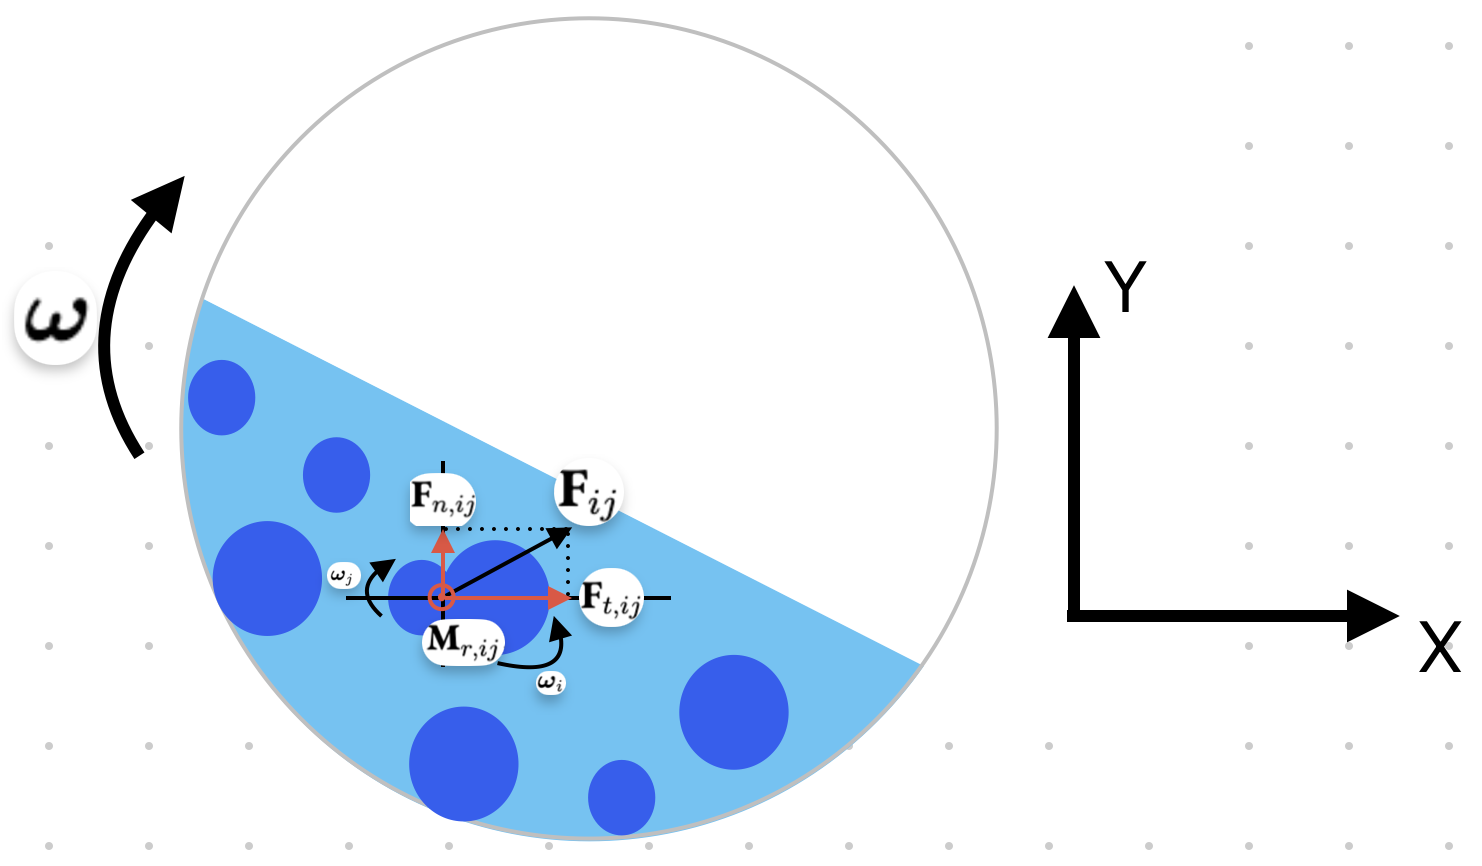
\includegraphics[width=\linewidth]{figures/principe_simulation_DEM.png}
\caption{Principe de la simulation DEM}
\end{figure}

\subsection{Du déterminisme particulaire au formalisme markovien}
% le but est de dire comment se construit un modèle de markov:
% ie le couple (Vecteur d'état initial, matrice de transition)
% Que traduit le vecteur initial d'état ?
% Quelle interpretation physique?
% Comment il se construit?
% Pareillement pour la matrice de transition

% Trouver une
%------------------
%% implementation  
%------------------

% Discrétisation
Plutôt que de suivre individuellement chaque grain, l'approche stochastique regroupe les particules dans des cellules issues d'une discrétisation spatiale de la zone utile mélangeur comme le montre la (figure~\ref{fig:maillage_melangeur}),
permettant de suivre l'évolution du mélange à l'échelle des cellules. Le modèle de markov est le couple vecteur initial d'état,et matrice de transition
\noindent
Des probabilités de saut entre cellules sont alors appliquées afin de reproduire la dynamique des particules dans le mélangeur sur une séries d'instants discrets. 
On considère l'état du mélangeur à un instant $t_i$ défini par le nombre de particules dans chaque cellule spatiale à l'aide d'un vecteur $\mathbf{S}$ : 


\begin{equation}
  \mathbf{S}(t_i)
  = 
  \begin{bmatrix}
    S_0(t_i)\\
    S_1(t_i)\\
    \vdots\\
    S_{N-1}(t_i)
  \end{bmatrix},
  % \qquad
  % S_i(t)
  % =
  % \begin{cases}
  %   N_i(t), & \text{mélange (comptage)},\\[4pt]
  %   c_i(t), & \text{ségrégation (teneur locale)}.
  % \end{cases}
  \label{eq:vecteur_etat}
\end{equation}
où $S_i(t_k)$ correspond au nombre de particules d'une espèce dans la cellule $ i \in [O,N-1]$ à l'instant $t_k$. À partir des probabilités de saut $\gamma_{j \to i}$ des cellules $j$ vers une cellule $i$, on peut calculer le nombre de particules dans la cellule $i$ à l'instant $t_{i+1}$ : 
\begin{align}
S_i(t_{k+1}) =\sum_{j=0}^{N-1}  \gamma_{j \to i}S_j(t_k)
\end{align}


Ce changement d'échelle autorise un pas de temps de prédiction nettement plus grand et un coût en ressources computationnelles réduit.
% On reconstruit ansi tout l'état du mélangeur à partir de la matrice de transition 

\begin{figure}[H]
  \centering
  \begin{minipage}{0.48\textwidth}
    \centering
    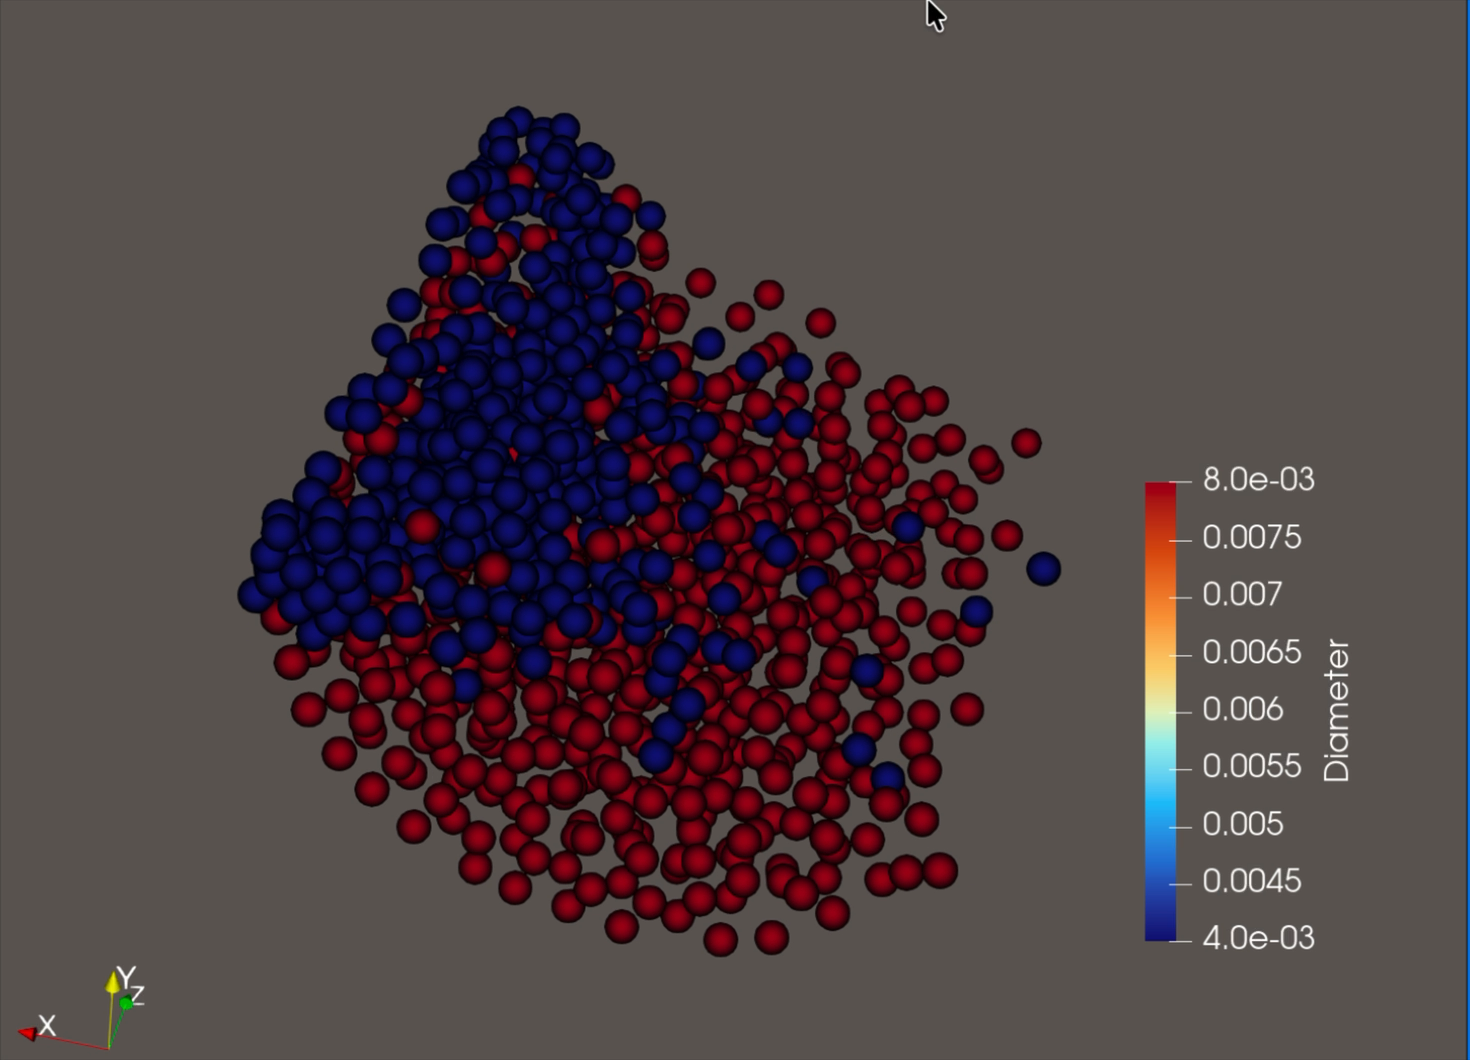
\includegraphics[width=\linewidth]{figures/melangeur_non_discretise.png}
    \subcaption*{(a) Mélangeur non discrétisé}
  \end{minipage}\hfill
  \begin{minipage}{0.48\textwidth}
    \centering
    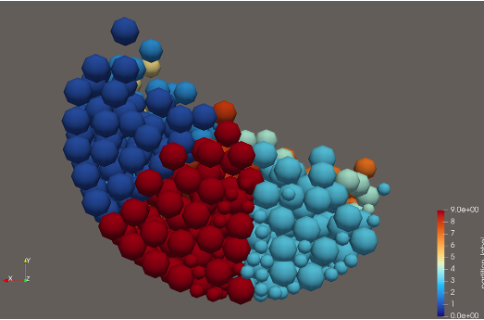
\includegraphics[width=\linewidth]{figures/melangeur_discretise.png}
    \subcaption*{(b) Mélangeur discrétisé}
  \end{minipage}
  \caption{Principe de la discrétisation spatiale : le tambour est partitionné en cellules au sein desquelles la dynamique particulaire est agrégée.}
  \label{fig:maillage_melangeur}
\end{figure}

% Durant une phase d'apprentissage, on observe les déplacements inter-cellules pour estimer la matrice de transition et initialiser le vecteur d'état $\mathbf{S}(0)$. La nature de ce vecteur dépend du phénomène que l'on souhaite caractériser :


% Le comptage $N_i(t)$ renseigne sur l'occupation globale du mélangeur ; la teneur locale $c_i(t)$, en revanche, discrimine les zones enrichies ou appauvries en une espèce donnée et se révèle plus adaptée à l'étude de la ségrégation.
\subsubsection{Construction du vecteur d'état initial}
Une fois le mélangeur discrétisé, chaque particule se voit attribué un label dependemment de son appartenance à une cellule. Differentes méthodes de discrétisation ont été dévéloppées pour éffectuer cette labélisation.
À l'issue de cette labélisaton, on obtient un vecteur de label $\mathbb{l}=
$
\subsubsection{Construction de la matrice de transition} 

La matrice de transition $\mathbf{P}$ encode la probabilité qu'une particule quitte la cellule source $j$ (colonne) pour rejoindre la cellule d'arrivée $i$ (ligne) durant un intervalle $\tau=t_{k+1}-t_k$, 
différence entre les instants $t_{k+1}$ et $t_k$  sur une période dite  \textbf{temps d'apprentissage} $t=NLT\times\tau$.
Ainsi donc, deux vecteurs d'états --$S_(t_{k+1})$ et $S_t_k$-- sont construits en les instants $t_{k+1}$ et $t_k$ respectivement

\begin{equation}
  P_{i,j}
  =
  \frac{1}{NLT}
  \sum_{n=1}^{NLT}
  \frac{1}{\phi(j,t_{n-1})}
  \sum_{p=1}^{N_p}
  \phi_p(i,t_n)\,
  \phi_p(j,t_{n-1}),
  \label{eq:matrice_transition}
\end{equation}

où $NLT$ est le nombre d'instants d'apprentissage, $\phi_p(i,t_n)$ la fonction indicatrice valant 1 si la particule $p$ occupe la cellule $i$ à l'instant $t_n$, et $\phi(j,t_{n-1})=\sum_p \phi_p(j,t_{n-1})$ le nombre total de grains dans la cellule $j$. La normalisation par $\phi(j,t_{n-1})$ assure le caractère stochastique en colonne :

\begin{equation}
  P_{ij} \geq 0,
  \qquad
  \sum_i P_{ij} = 1.
  \label{eq:stochastique}
\end{equation}

\paragraph{Chaîne homogène.} Lorsque $\mathbf{P}$ est supposée invariante dans le temps, la prédiction à $n$ pas s'écrit :

\begin{equation}
  \mathbf{S}(t+n\Delta t)
  =
  \mathbf{P}^n \, \mathbf{S}(t).
  \label{eq:prediction_homogene}
\end{equation}

\paragraph{Chaîne inhomogène.} Pour capturer l'évolution temporelle des probabilités, on estime une séquence de matrices $\{\mathbf{P}^{(k)}\}$ et la prédiction devient :

\begin{equation}
  \mathbf{S}_{k+1}
  =
  \mathbf{P}^{(k)} \, \mathbf{S}_k.
  \label{eq:prediction_inhomogene}
\end{equation}

\begin{figure}[H]
  \centering
  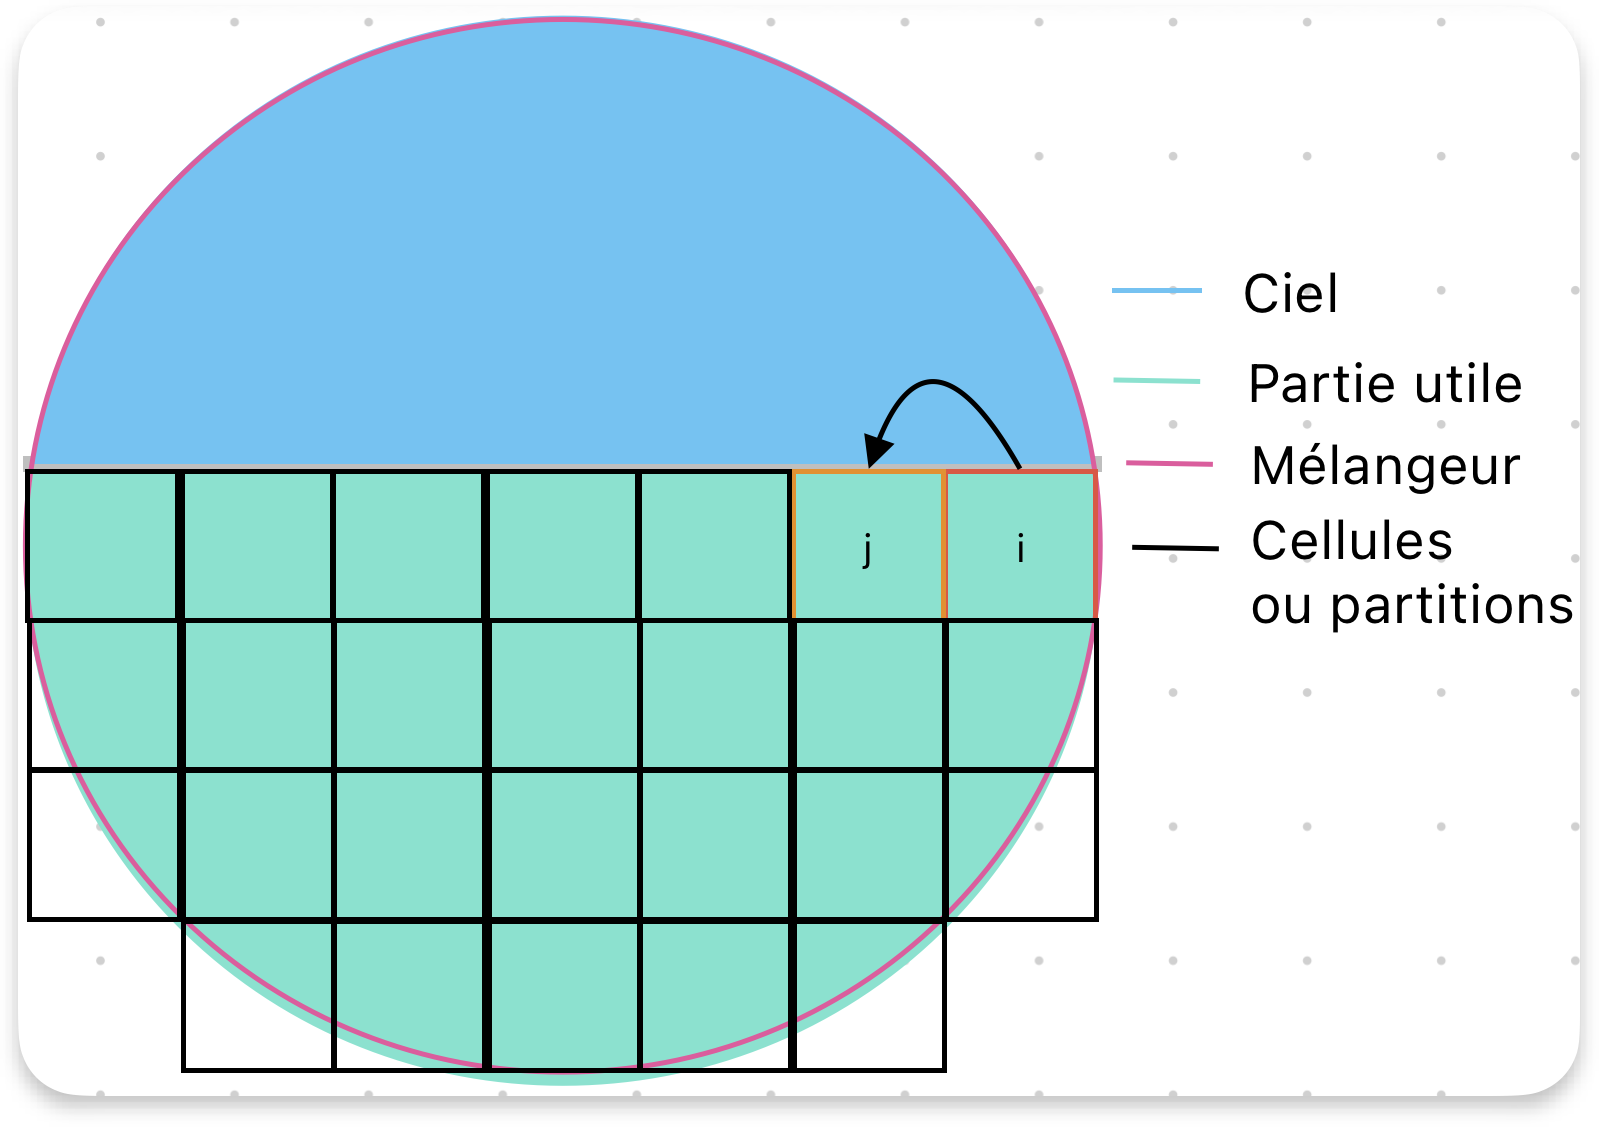
\includegraphics[width=0.75\textwidth]{figures/representation_melangeur.png}
  \caption{Construction de la matrice de transition à partir des déplacements inter-cellules observés dans le mélangeur discrétisé.}
  \label{fig:representation_melangeur}
\end{figure}

\begin{figure}[H]
  \centering
  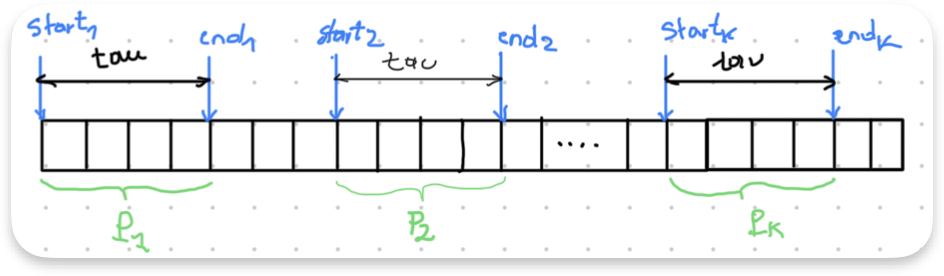
\includegraphics[width=0.85\textwidth]{figures/representation_chaine_inhomogene.png}
  \caption{Principe de la chaîne inhomogène : une matrice de transition distincte est associée à chaque intervalle de temps.}
  \label{fig:representation_chaine_inhomogene}
\end{figure}

% ============================================================
% MÉTHODES DE DISCRÉTISATION
% ============================================================
\subsubsection{Méthodes de discrétisation}

Plusieurs stratégies de maillage ont été développées ou testées durant le stage. Elles se répartissent en deux familles :

\begin{itemize}[itemsep=3pt]
  \item \textbf{Méthodes géométriques}, fondées sur la géométrie des cellules, elles permettent d'avoir des volumes égaux.

    \begin{itemize}
      \item découpage cartésien ;
      \item découpage cylindrique.
    \end{itemize}
  \item \textbf{Méthodes statistiques}, fondées sur la distribution effective des particules et des grandeurs physiques associées :
    \begin{itemize}
      \item découpage quantile ;
      \item découpage de Voronoï ;
      \item découpage physique ;
      \item découpage adaptatif ;
      \item découpage par mélange gaussien ;
      \item découpage par clustering spectral ;
      \item découpage multizone ;
      \item découpage octree.
    \end{itemize}
\end{itemize}

Quelle que soit la méthode retenue, une phase d'apprentissage sur le régime permanent est nécessaire pour caler les frontières des cellules et éviter de créer des partitions vides.

\paragraph{Découpage cartésien}
Les cellules obtenues sont des parallélépipèdes rectangles de volume constant.
Le mélangeur est segmenté selon les trois axes $x$, $y$, $z$ en un nombre fixé d'intervalles. Chaque particule reçoit un label correspondant à la cellule dans laquelle elle se trouve. La numérotation globale suit l'ordre lexicographique $x \to y \to z$.

\paragraph{Découpage cylindrique}
Les cellules obtenues sont des tranches cylindriques pleins.
Un changement de coordonnées est d'abord opéré :

\begin{equation}
  r = \sqrt{x^2 + y^2},
  \qquad
  \theta = \operatorname{atan2}(y,x),
  \qquad
  z = z.
  \label{eq:cylindrique}
\end{equation}

Les particules sont ensuite affectées à des cellules définies par des intervalles en $r$, $\theta$ et $z$. La numérotation globale suit l'ordre radial $\to$ angulaire $\to$ axial. Ce découpage épouse naturellement la géométrie du tambour.

\paragraph{Découpage de Voronoï par algorithme des k-moyennes}
\label{sec:voronoi_kmeans}

Le découpage de Voronoï est obtenu à l'aide d'un algorithme de partitionnement de type k-moyennes (\textit{k-means}). L'objectif est de regrouper les particules en $K$ cellules de manière à minimiser la dispersion des observations à l'intérieur de chaque cellule. Chaque cellule est ensuite associée à un centroïde, c'est-à-dire un point représentatif autour duquel les particules sont affectées.

La fonction objectif minimisée par l'algorithme est la variance intra-cellule :

\begin{equation}
  J
  =
  \sum_{k=1}^{K}
  \sum_{p \in \mathcal{C}_k}
  \left\|
    \mathbf{z}_p - \boldsymbol{\mu}_k
  \right\|^2,
  \label{eq:kmeans}
\end{equation}

où $\mathbf{z}_p$ désigne le vecteur position de la particule $p$, $\boldsymbol{\mu}_k$ le centre de la cellule $k$, et $\mathcal{C}_k$ l'ensemble des particules affectées à cette cellule. Dans le cas du découpage de Voronoï purement spatial, le vecteur $\mathbf{z}_p$ contient uniquement les coordonnées de la particule :

\[
  \mathbf{z}_p =
  \begin{bmatrix}
    x_p & y_p & z_p
  \end{bmatrix}^T .
\]

L'algorithme fonctionne de manière itérative en alternant deux étapes principales : une étape d'affectation des particules aux cellules, puis une étape de mise à jour des centres.

\subparagraph{Initialisation des centres.} 
Les centres initiaux $\boldsymbol{\mu}_k^{(0)}$ sont choisis aléatoirement parmi les échantillons disponibles, c'est-à-dire parmi les positions des particules observées pendant la phase d'apprentissage. Ce choix aléatoire peut toutefois influencer la configuration finale de la partition, car l'algorithme peut converger vers différents minima locaux selon la position initiale des centres.

Afin de limiter cette dépendance et d'améliorer la robustesse du maillage, la procédure est répétée pour dix initialisations différentes. Autrement dit, dix configurations initiales distinctes sont construites, puis les modèles obtenus sont consolidés par moyenne. Cette stratégie permet de réduire l'effet d'un tirage initial défavorable et de produire une partition plus représentative de la distribution globale des particules.

\subparagraph{Étape d'affectation.}
À l'itération $q$, chaque particule est affectée à la cellule dont le centre est le plus proche au sens de la distance euclidienne dans l'espace des caractéristiques :

\begin{equation}
  \mathcal{C}_k^{(q)}
  =
  \left\{
    p \; : \;
    \left\|
      \mathbf{z}_p - \boldsymbol{\mu}_k^{(q)}
    \right\|
    \leq
    \left\|
      \mathbf{z}_p - \boldsymbol{\mu}_\ell^{(q)}
    \right\|,
    \quad
    \forall \ell \neq k
  \right\}.
  \label{eq:affectation_kmeans}
\end{equation}

Ainsi, une particule appartient à la cellule $k$ si la distance entre cette particule et le centre $\boldsymbol{\mu}_k$ est inférieure ou égale à sa distance à tout autre centre $\boldsymbol{\mu}_\ell$. La figure~\ref{fig:centres_voronoi} illustre cette règle d'affectation : chaque grain est attribué à la partition dont le centroïde est le plus proche.

\begin{figure}[H]
  \centering
  \begin{minipage}{0.85\textwidth}
    \centering
    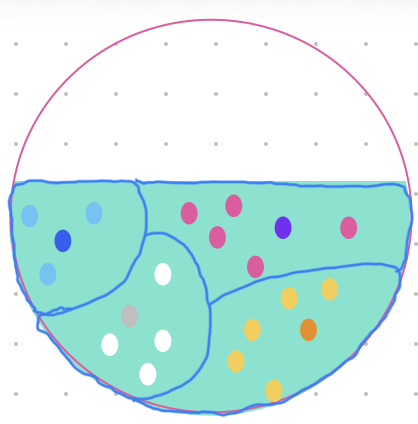
\includegraphics[width=\linewidth]{figures/centres_voronoi.png}
  \end{minipage}
  \caption{Attribution des particules aux cellules de Voronoï : à l'issue de la phase d'apprentissage, chaque grain est affecté à la partition dont le centre $\boldsymbol{\mu}_k$ est le plus proche au sens de la distance euclidienne (équation~\ref{eq:affectation_kmeans}).}
  \label{fig:centres_voronoi}
\end{figure}

\subparagraph{Étape de mise à jour.}
Une fois les particules affectées aux différentes cellules, les centres sont recalculés comme la moyenne des caractéristiques des particules appartenant à chaque cellule :

\begin{equation}
  \boldsymbol{\mu}_k^{(q+1)}
  =
  \frac{1}{\left|\mathcal{C}_k^{(q)}\right|}
  \sum_{p \in \mathcal{C}_k^{(q)}}
  \mathbf{z}_p ,
  \label{eq:update_kmeans}
\end{equation}

où $\left|\mathcal{C}_k^{(q)}\right|$ représente le nombre de particules affectées à la cellule $k$ à l'itération $q$. Cette mise à jour déplace les centres vers les zones de plus forte densité d'observations, ce qui permet d'affiner progressivement la partition.

\subparagraph{Convergence et critère d'arrêt.}
La procédure est appliquée de manière récursive jusqu'à ce qu'un critère de convergence soit satisfait. La variance intra-cellule est recalculée à chaque itération :

\begin{equation}
  J^{(q)}
  =
  \sum_{k=1}^{K}
  \sum_{p \in \mathcal{C}_k^{(q)}}
  \left\|
    \mathbf{z}_p - \boldsymbol{\mu}_k^{(q)}
  \right\|^2 .
  \label{eq:variance_kmeans}
\end{equation}

L'algorithme est arrêté lorsque l'une des deux conditions suivantes est remplie :

\begin{itemize}[itemsep=2pt]
  \item la variance, ou sa variation relative entre deux itérations successives, devient inférieure ou égale à un seuil fixé ;
  \item le nombre maximal d'itérations est atteint.
\end{itemize}

Dans les présents calculs, la variance seuil est fixée à $0{,}0001$ et le nombre maximal d'itérations est limité à $300$. Cette double condition permet à la fois d'interrompre l'algorithme lorsque la partition est suffisamment stable, et d'éviter un temps de calcul excessif dans les cas où la convergence serait lente.

Une fois les centres convergés, les cellules de Voronoï sont définies à partir de ces centres. Chaque particule est alors associée à la cellule correspondant au centroïde le plus proche. Ce découpage permet d'obtenir des cellules adaptées à la distribution effective des particules, contrairement à un maillage purement géométrique qui ne tient pas compte de leur occupation réelle du mélangeur.
\paragraph{Découpage physique} 
Le découpage physique repose sur le même algorithme de k-moyennes que le découpage de Voronoï. La seule différence provient du vecteur de caractéristiques $\mathbf{z}_p$, qui est enrichi par une grandeur cinématique représentative de la dynamique locale : la norme de la vitesse de la particule. La partition n'est donc plus uniquement construite à partir de la position des grains, mais également à partir de leur mobilité.

\begin{equation}
  \mathbf{z}_p
  =
  \begin{bmatrix}
    x_p & y_p & z_p & \|\mathbf{v}_p\|
  \end{bmatrix}^T.
  \label{eq:physics}
\end{equation}

% L'algorithme de partitionnement reste un k-means, mais opéré dans un espace de dimension quatre. La figure~\ref{fig:schematisation_voronoi_physique} illustre visuellement l'application des découpages de Voronoï et physique sur les données DEM.

\begin{figure}[H]
  \centering
  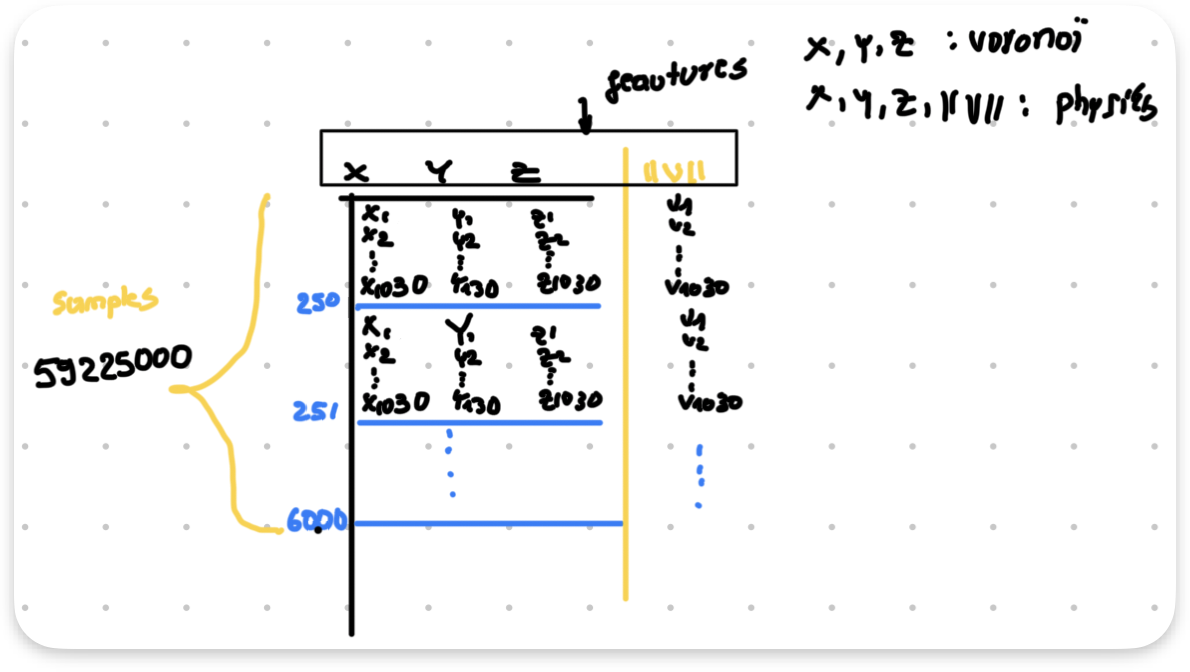
\includegraphics[width=0.85\textwidth]{figures/schematisation_voronoi_physique.png}
  \caption{Application des découpages de Voronoï et physique aux positions issues de la simulation DEM.}
  \label{fig:schematisation_voronoi_physique}
\end{figure}

% ============================================================
% RÉSULTATS
% ============================================================

\section{Résultats}
\label{sec:resultats}

Cette section expose les résultats obtenus pour les trois principales méthodes de discrétisation. Pour quantifier le degré d'homogénéité, nous utilisons l'écart-type relatif (\textit{Relative Standard Deviation}, RSD) :

\begin{equation}
  \mathrm{RSD}(t)
  =
  \frac{
    \sqrt{
      \frac{1}{N_c}
      \sum_{i=1}^{N_c}
      \left(
        c_i(t) - \bar{c}
      \right)^2
    }
  }{
    \bar{c}
  },
  \label{eq:rsd}
\end{equation}

où $N_c$ est le nombre de cellules et $\bar{c}$ la teneur moyenne en petites particules.

\subsection{Découpage cartésien}

Les matrices de transition (figure~\ref{fig:matrice_cartesien}) révèlent d'emblée une asymétrie marquée entre les deux espèces : les grandes particules présentent une probabilité diagonale élevée, signe d'une faible mobilité, tandis que les petites particules se redistribuent plus largement d'une cellule à l'autre.

\begin{figure}[H]
  \centering
  \begin{minipage}{0.48\textwidth}
    \centering
    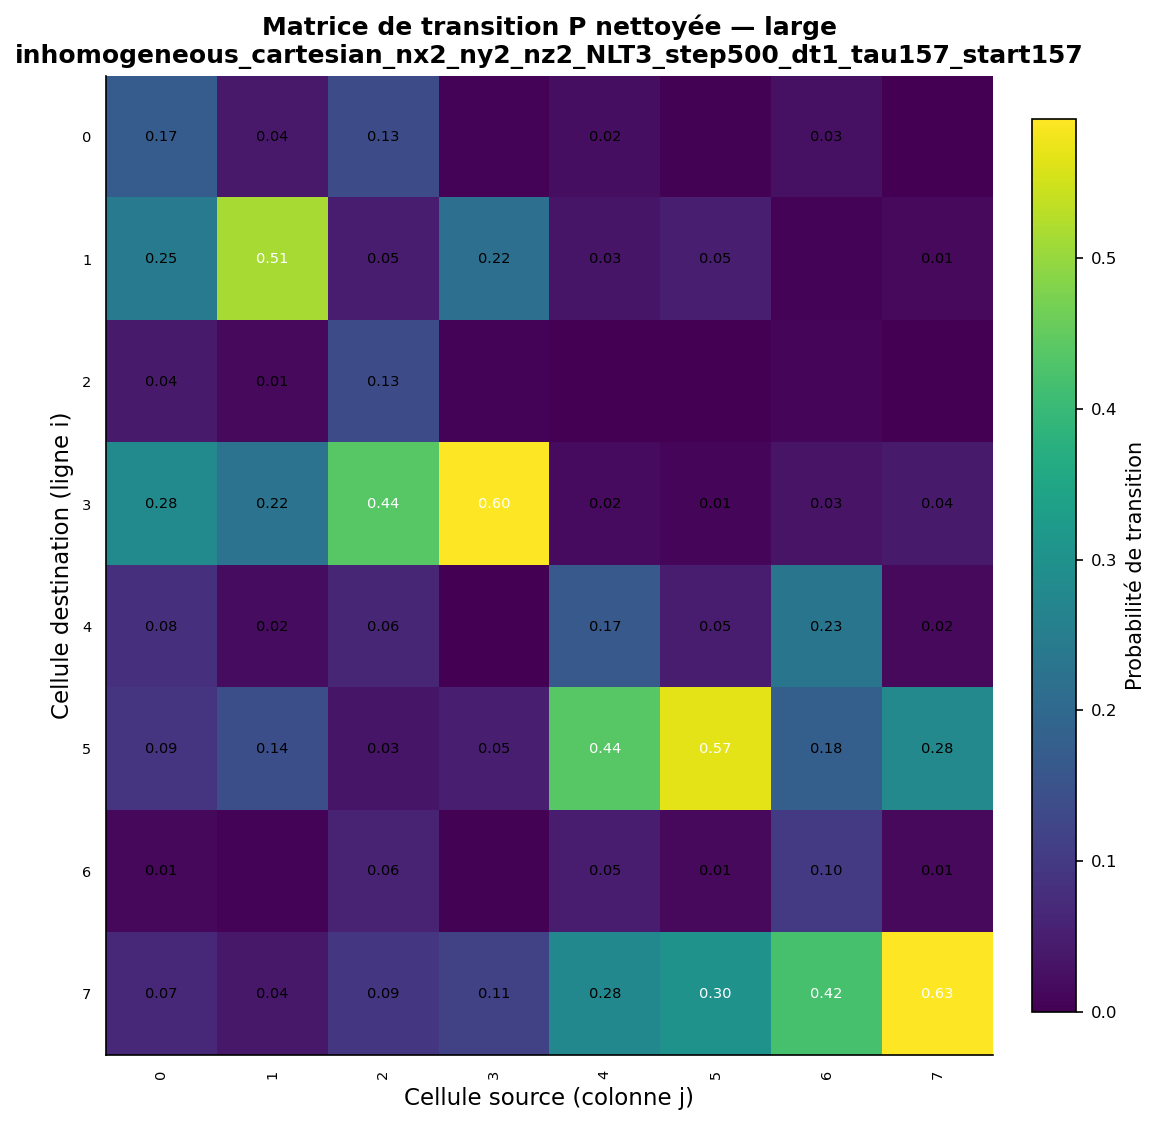
\includegraphics[width=\linewidth]{figures/matrice_cartesien_grandes.png}
    \subcaption*{(a) Grandes particules}
  \end{minipage}\hfill
  \begin{minipage}{0.48\textwidth}
    \centering
    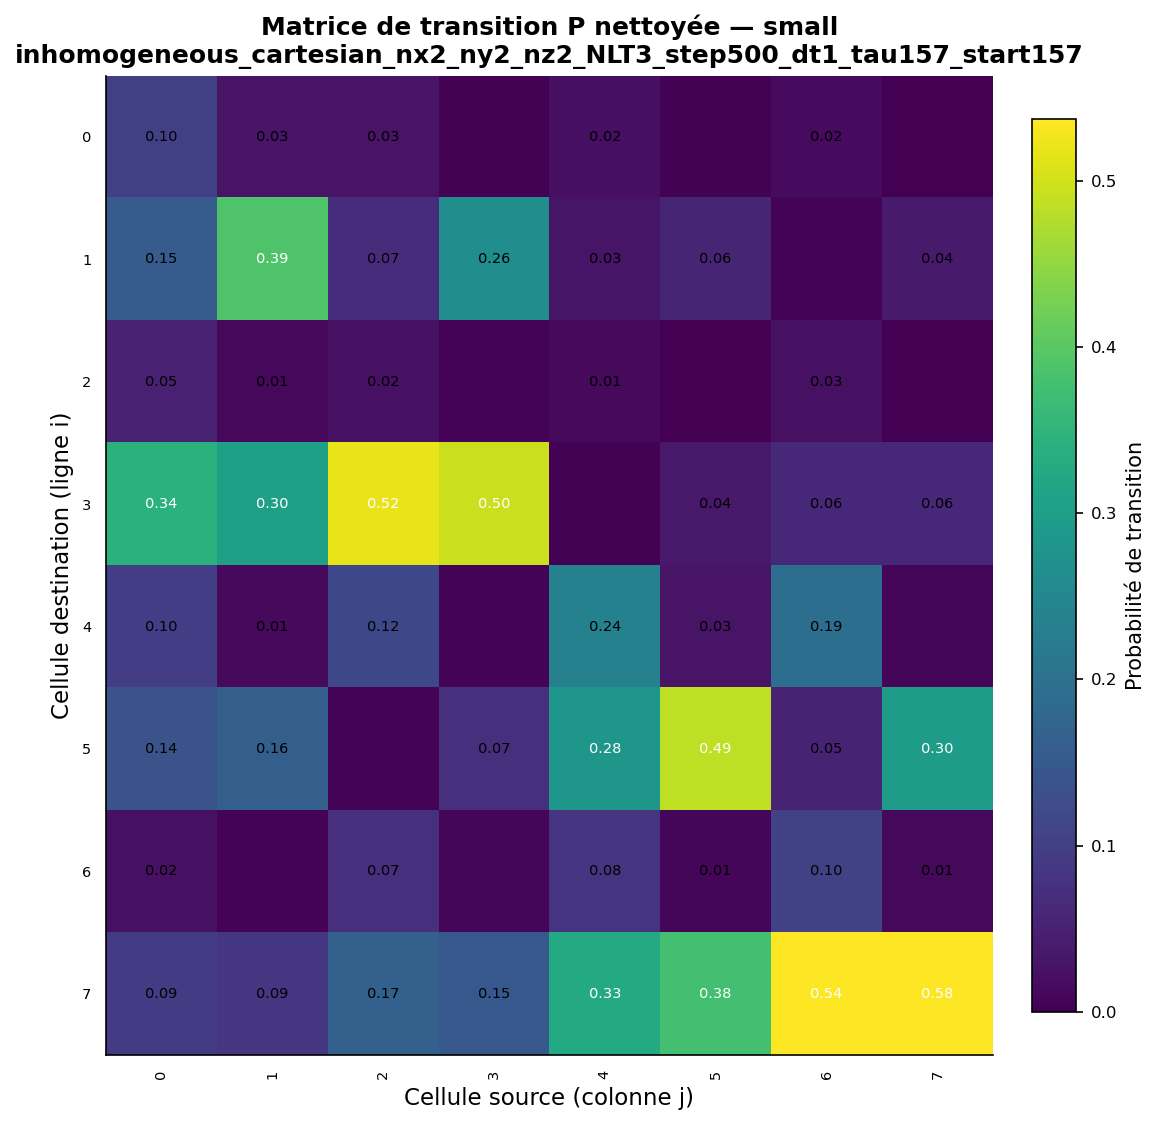
\includegraphics[width=\linewidth]{figures/matrice_cartesien_petites.png}
    \subcaption*{(b) Petites particules}
  \end{minipage}
  \caption{Matrices de transition (découpage cartésien) construites séparément pour chaque espèce.}
  \label{fig:matrice_cartesien}
\end{figure}

L'évolution du nombre total de particules par cellule fait apparaître des zones nettement sur-concentrées et d'autres quasi vides, confirmant qu'un simple comptage reste insuffisant pour caractériser la ségrégation.

\subsection{Découpage de Voronoï}

Le pas de temps markovien est fixé à \SI{1.57}{s}, soit approximativement un tour complet du tambour. Avec 10 cellules, le nombre moyen de particules par cellule avoisine 100, garantissant une statistique robuste.

Deux matrices distinctes sont estimées en appliquant un masque sur les labels afin d'isoler chaque espèce. La probabilité maximale de transition inter-cellule atteint $\approx 0{,}5$ pour les grandes particules contre $\approx 0{,}35$ pour les petites, confirmant la mobilité supérieure de ces dernières (figure~\ref{fig:matrices_voronoi}).

\begin{figure}[H]
  \centering
  \begin{minipage}{0.45\textwidth}
    \centering
    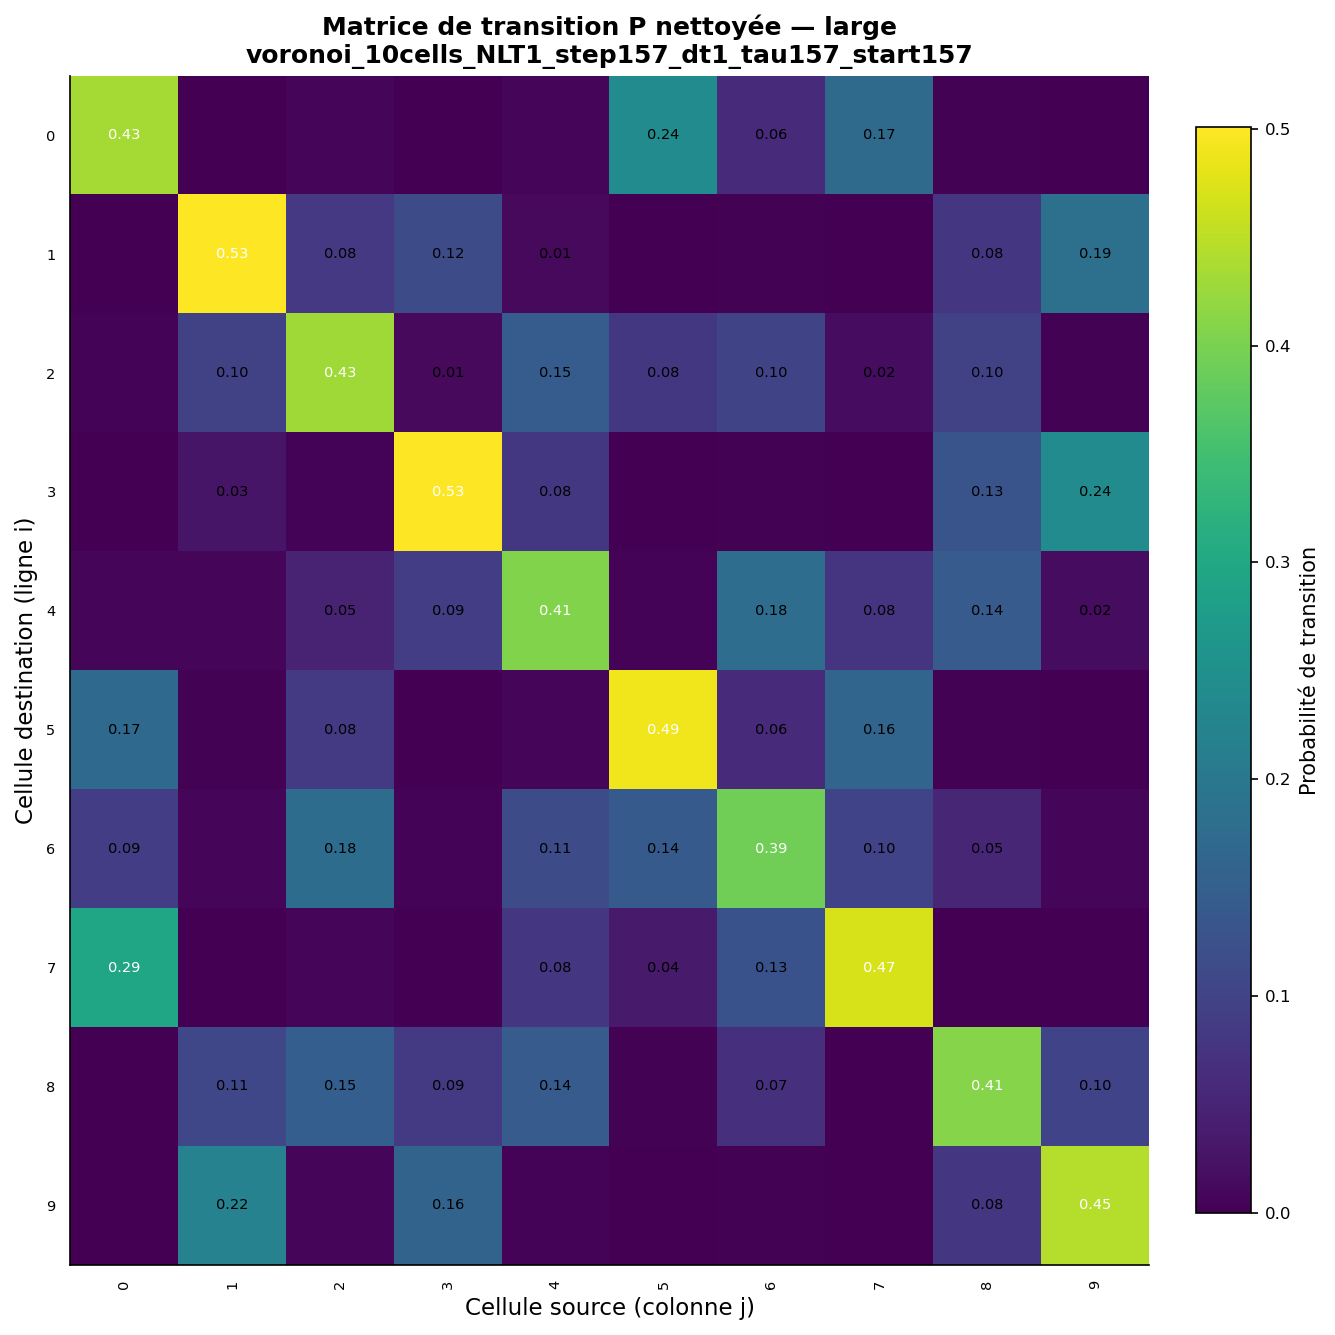
\includegraphics[width=\linewidth]{figures/voronoi_grandes.png}
    \subcaption*{(a) Grandes particules}
  \end{minipage}\hfill
  \begin{minipage}{0.45\textwidth}
    \centering
    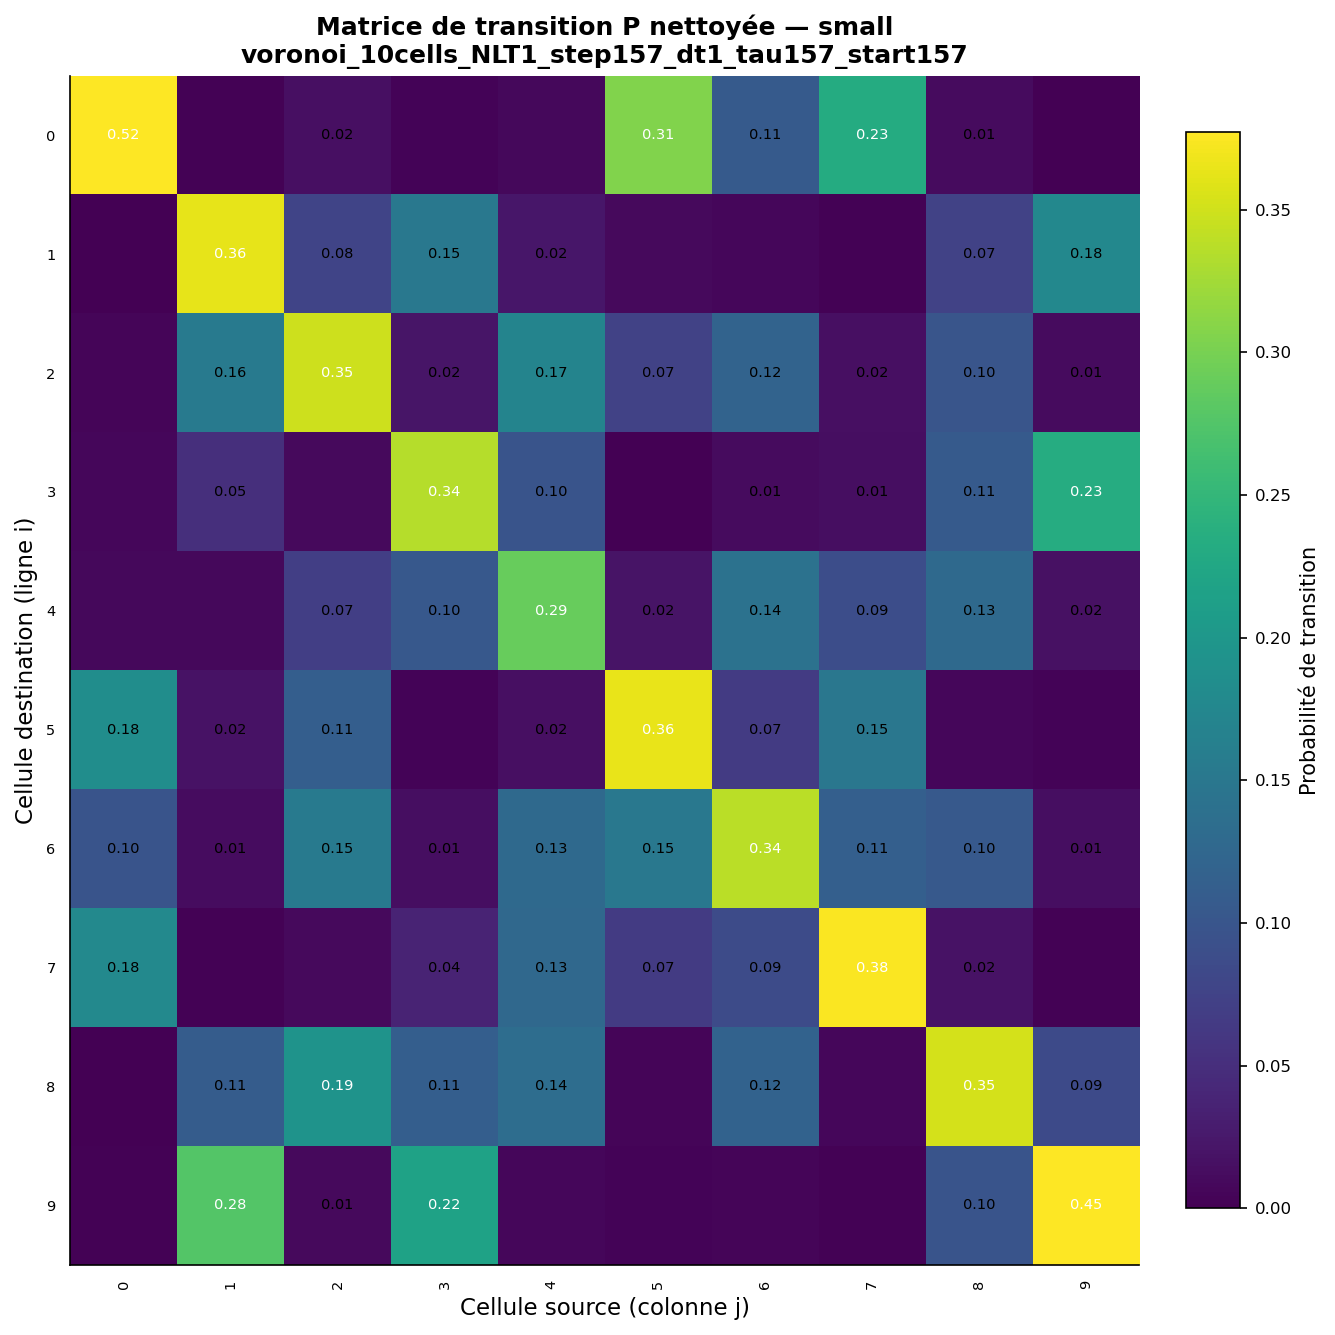
\includegraphics[width=\linewidth]{figures/voronoi_petites.png}
    \subcaption*{(b) Petites particules}
  \end{minipage}
  \caption{Matrices de transition (découpage de Voronoï) pour chaque espèce.}
  \label{fig:matrices_voronoi}
\end{figure}

\paragraph{Vecteur d'état par comptage.} La figure~\ref{fig:vecteur_etat_nb} montre l'évolution du nombre de particules par cellule. Si cette représentation décrit l'occupation globale du tambour, elle ne permet pas de discriminer les zones enrichies en une espèce.

\begin{figure}[H]
  \centering
  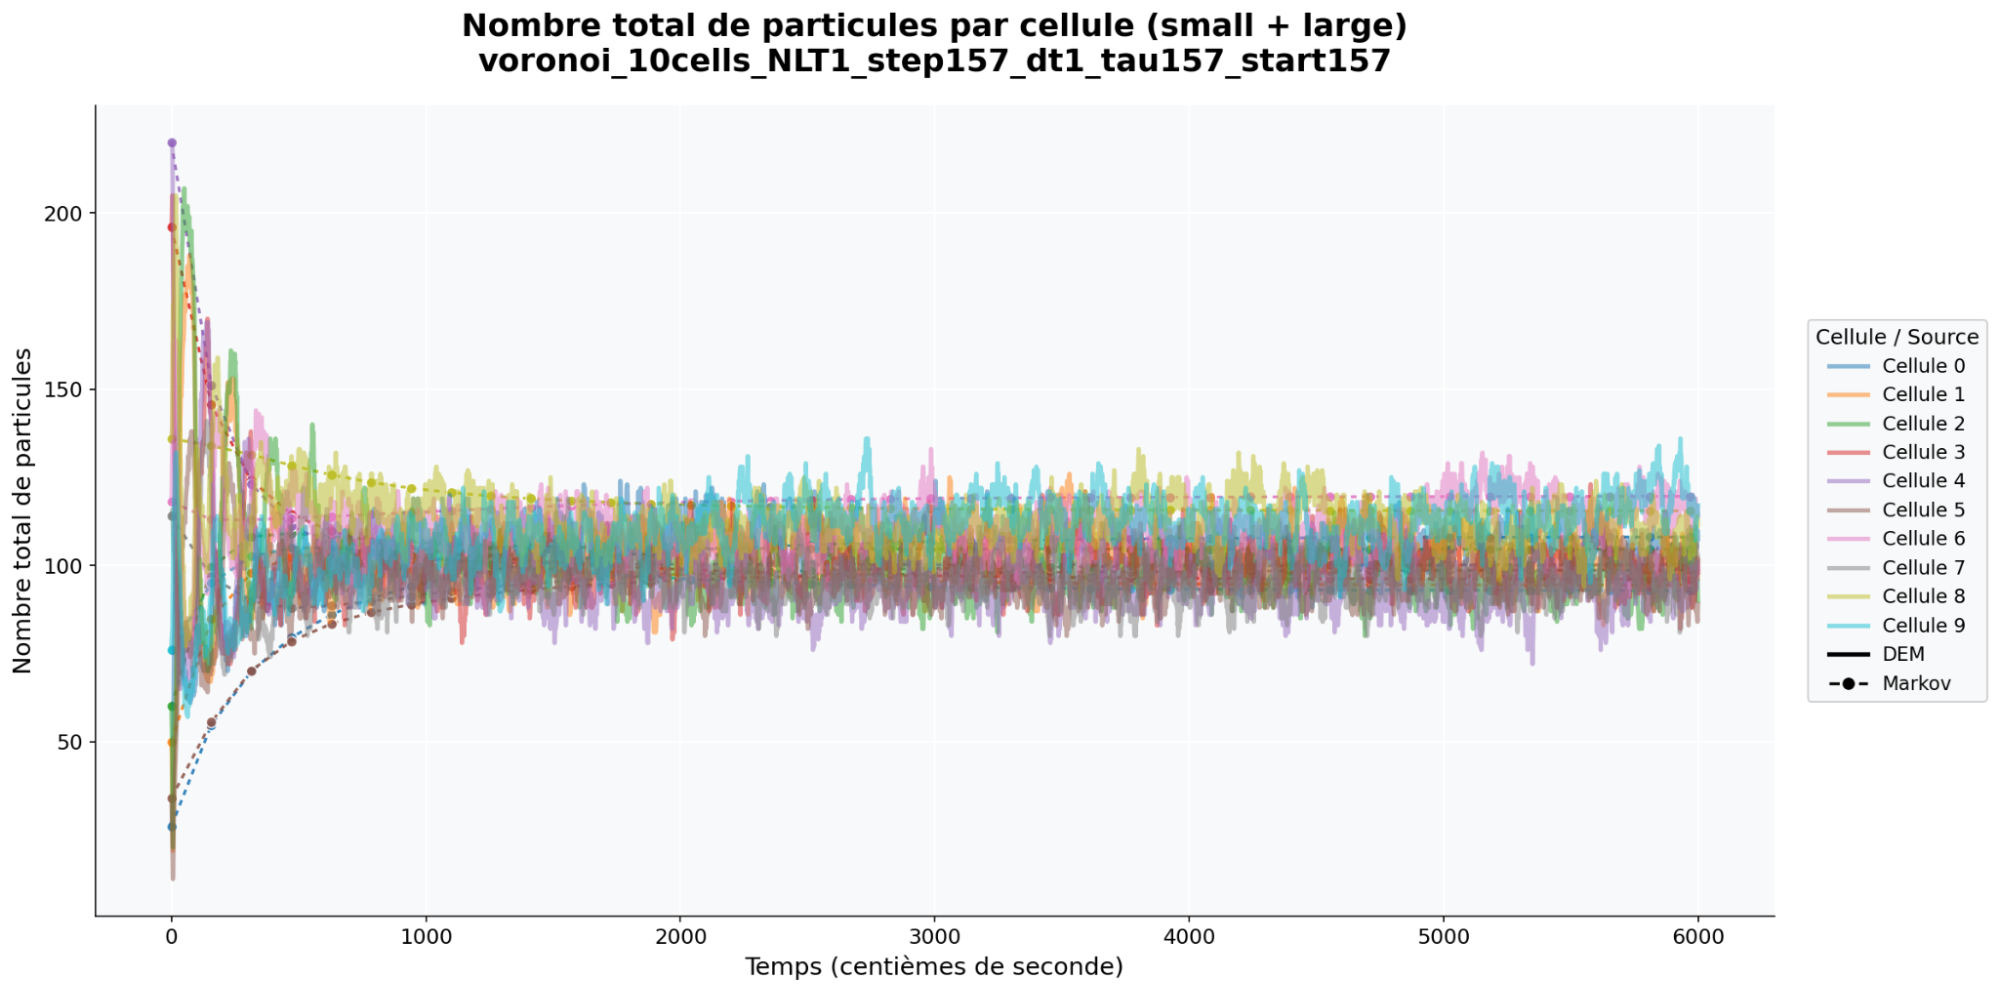
\includegraphics[width=0.85\textwidth]{figures/vecteur_etat_nb.png}
  \caption{Évolution temporelle du nombre de particules par cellule (vecteur d'état de type comptage).}
  \label{fig:vecteur_etat_nb}
\end{figure}

\paragraph{Vecteur d'état par teneur locale.} En substituant au comptage la teneur en petites particules, des écarts significatifs entre cellules émergent (figure~\ref{fig:teneur_petites}) : la cellule 9, adossée à la paroi, s'enrichit en petits grains tandis que la cellule 4 s'appauvrit. Cette hétérogénéité, invisible dans le comptage, traduit la ségrégation en cours.

\begin{figure}[H]
  \centering
  \begin{minipage}{0.48\textwidth}
    \centering
    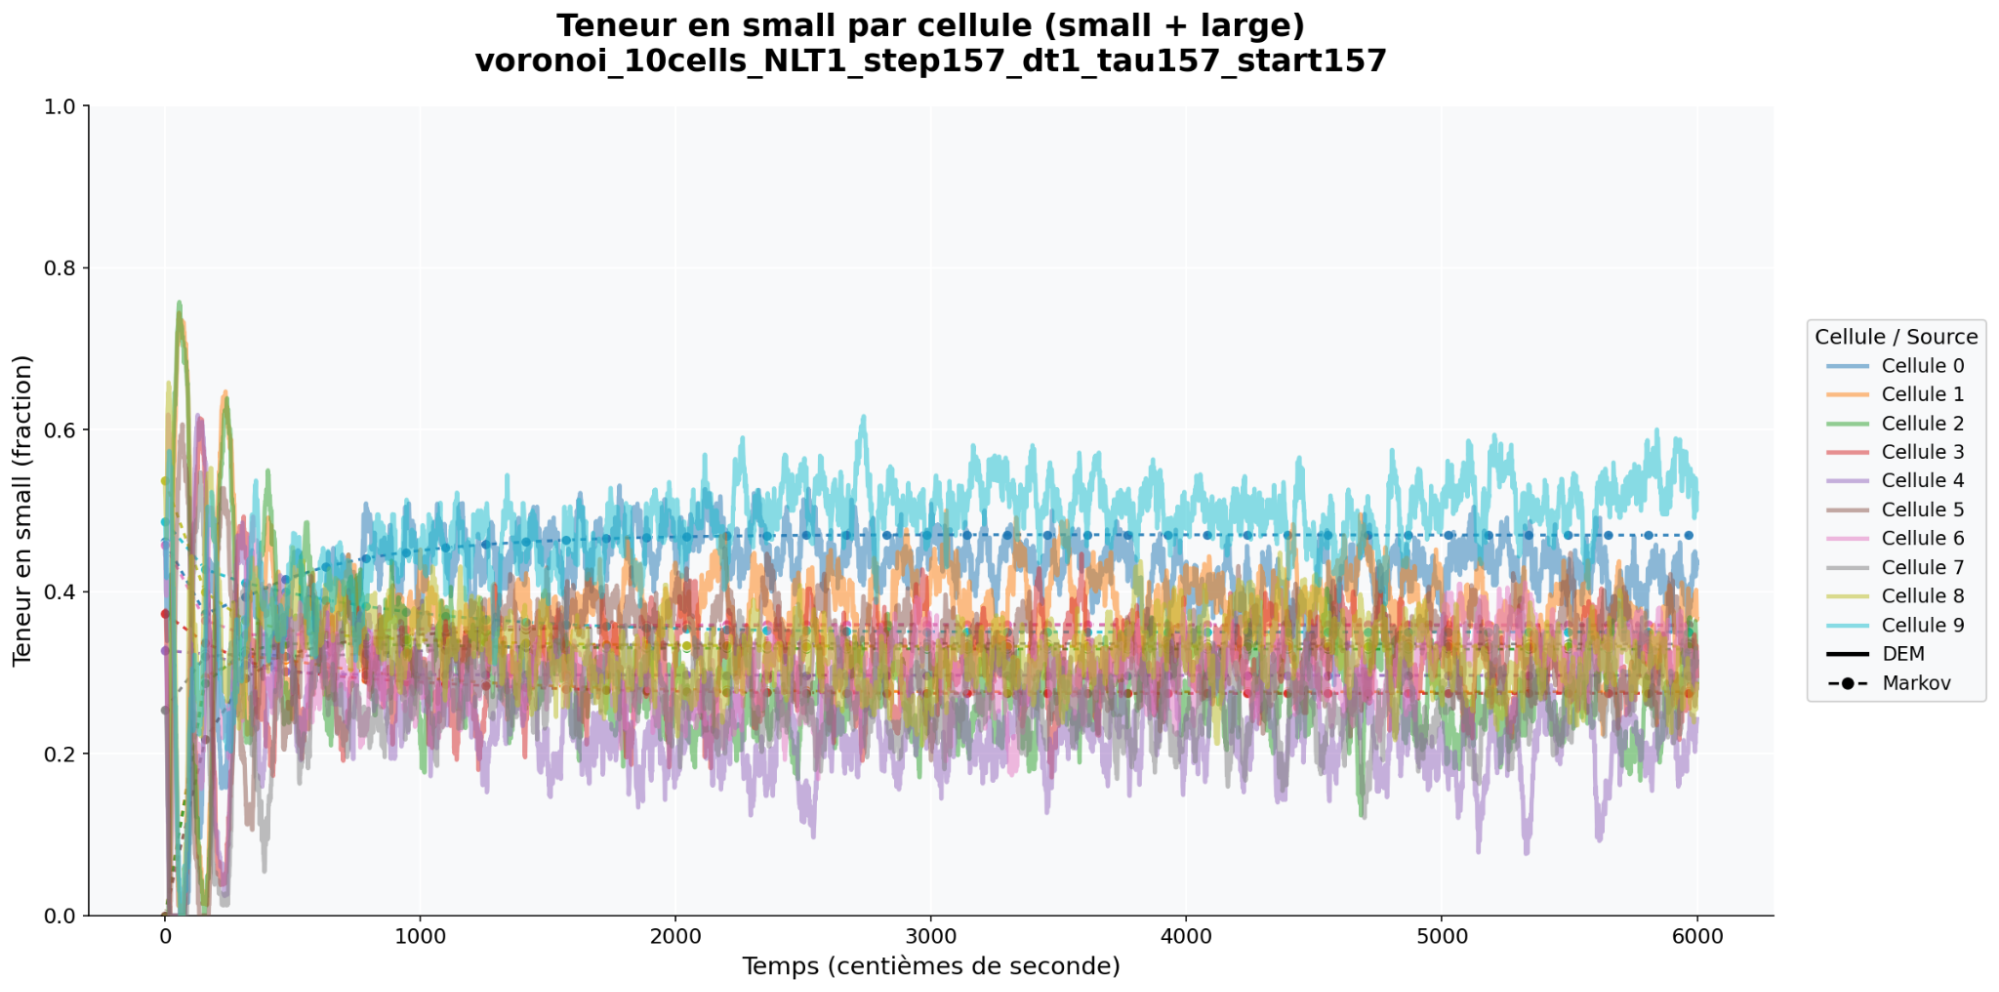
\includegraphics[width=\linewidth]{figures/teneur_petites1.png}
    \subcaption*{(a) Teneur en petites particules}
  \end{minipage}\hfill
  \begin{minipage}{0.48\textwidth}
    \centering
    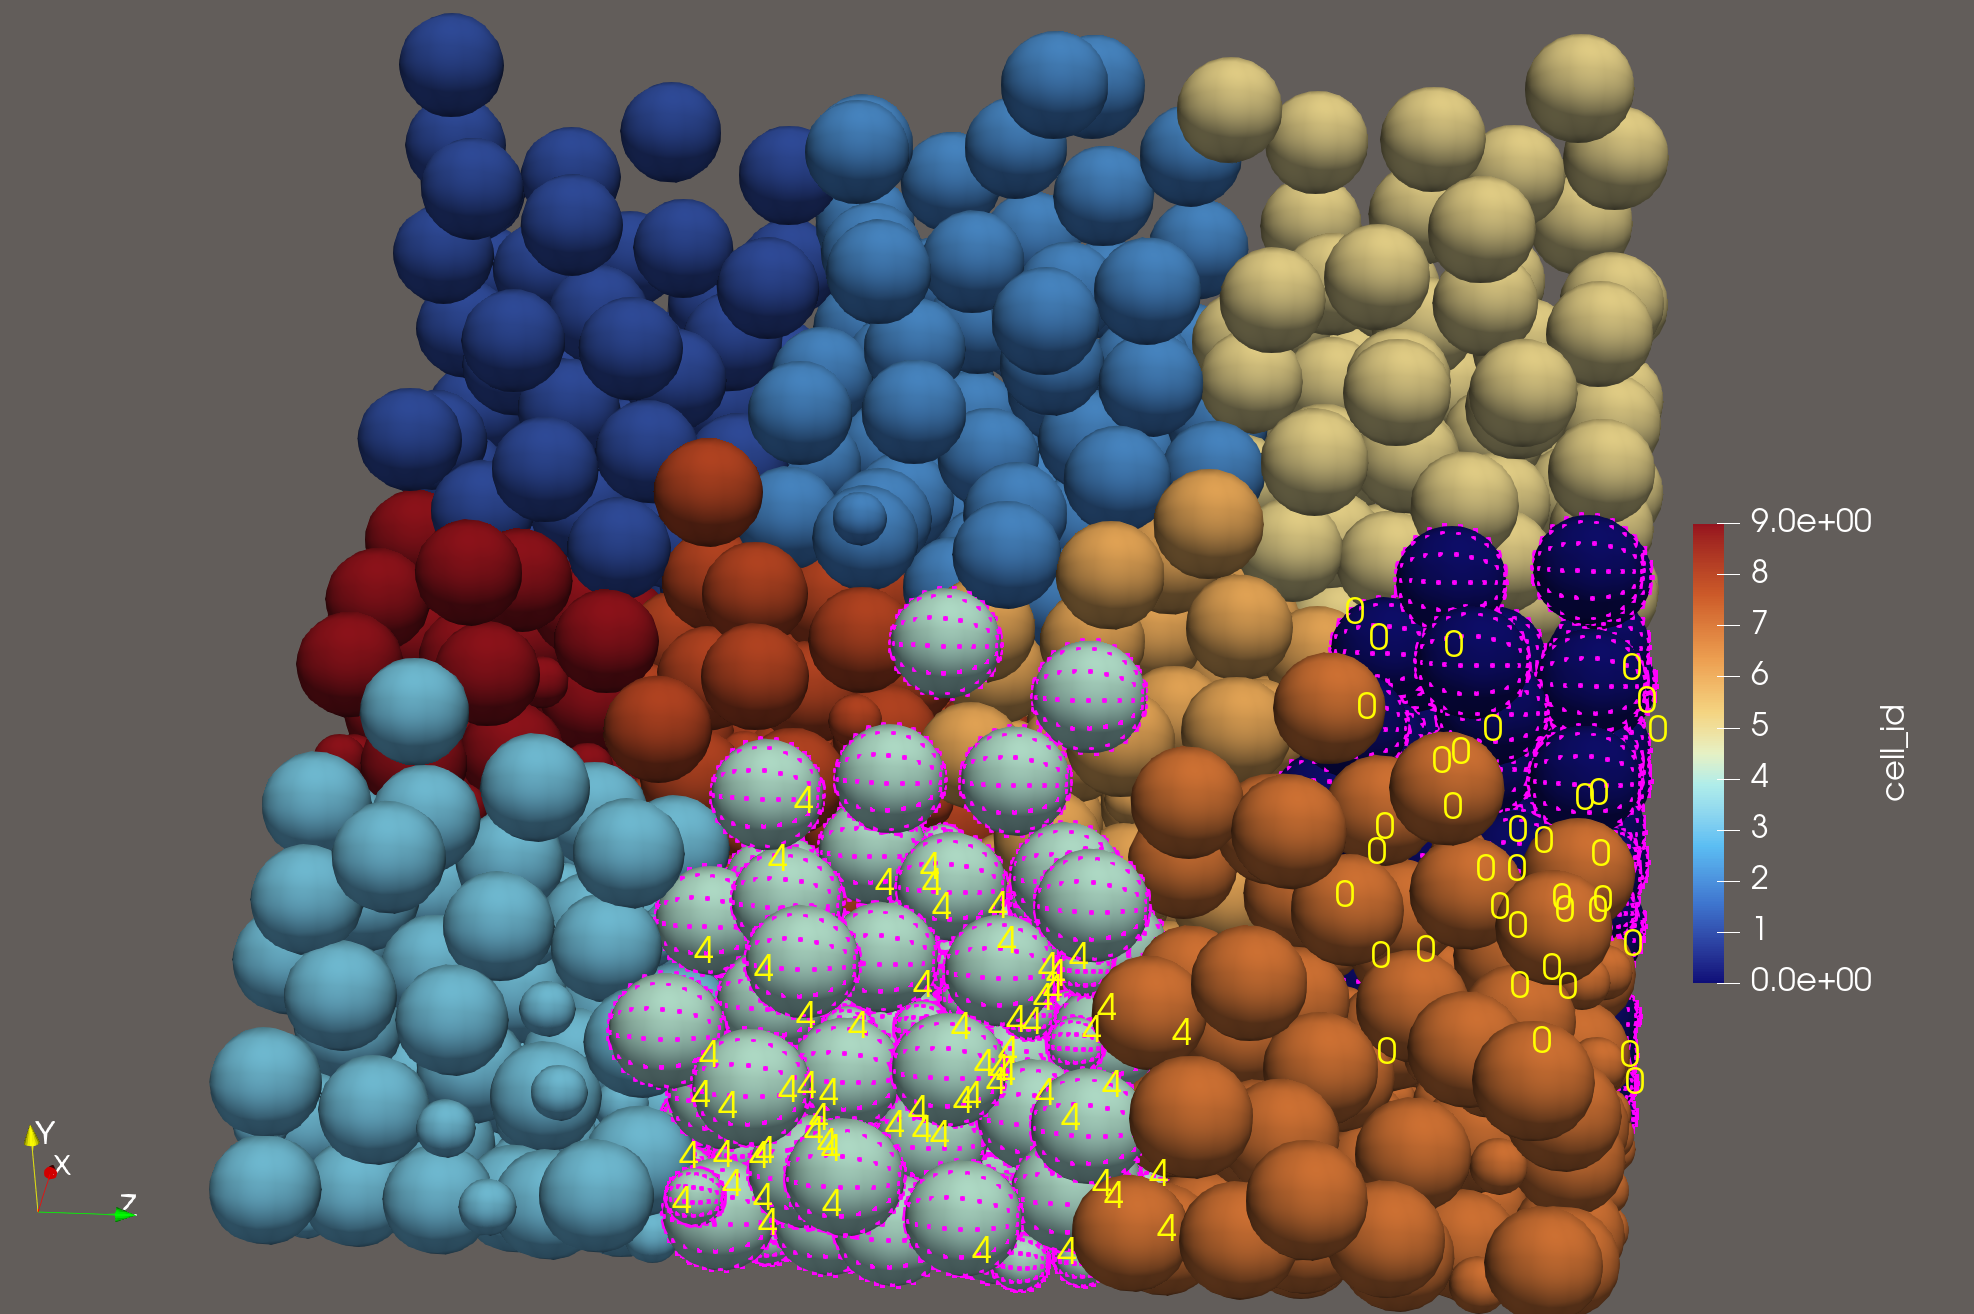
\includegraphics[width=\linewidth]{figures/teneur_petites2.png}
    \subcaption*{(b) Vue d'ensemble}
  \end{minipage}
  \caption{Évolution de la teneur locale en petites particules (vecteur d'état de type ségrégation).}
  \label{fig:teneur_petites}
\end{figure}

\paragraph{Validation par le RSD.} La figure~\ref{fig:rsd_voronoi} compare le RSD issu de la DEM à celui prédit par la chaîne de Markov. L'accord qualitatif confirme que le modèle reproduit correctement le niveau global d'homogénéisation atteint par le système.

\begin{figure}[H]
  \centering
  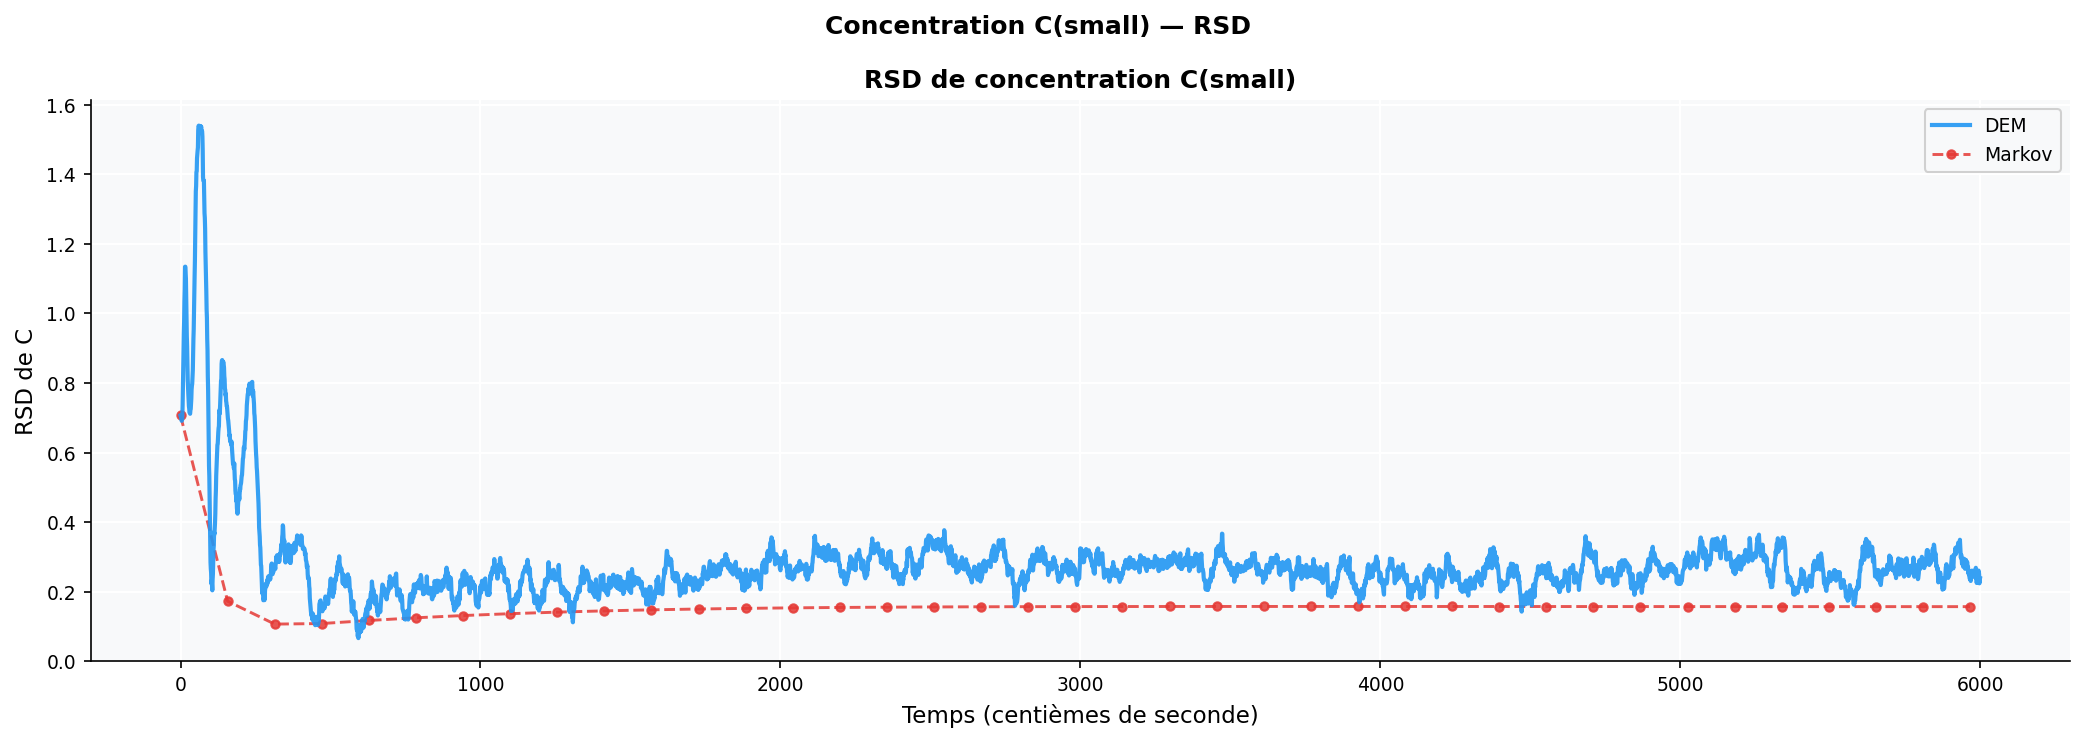
\includegraphics[width=0.85\textwidth]{figures/rsd_voronoi.png}
  \caption{RSD de la concentration en petites particules : comparaison DEM / prédiction markovienne (découpage de Voronoï).}
  \label{fig:rsd_voronoi}
\end{figure}

\subsection{Découpage physique et chaînes inhomogènes}

En intégrant la norme de la vitesse dans le critère de partitionnement, les cellules formées dans la zone passive reçoivent davantage de particules et exhibent une probabilité diagonale nettement plus élevée --- signature du piégeage temporaire des grains dans le cœur du lit. À l'inverse, les cellules de la zone active, plus agitées, présentent des transitions plus diffuses (figure~\ref{fig:matrice_physique}).

\begin{figure}[H]
  \centering
  \begin{minipage}{0.48\textwidth}
    \centering
    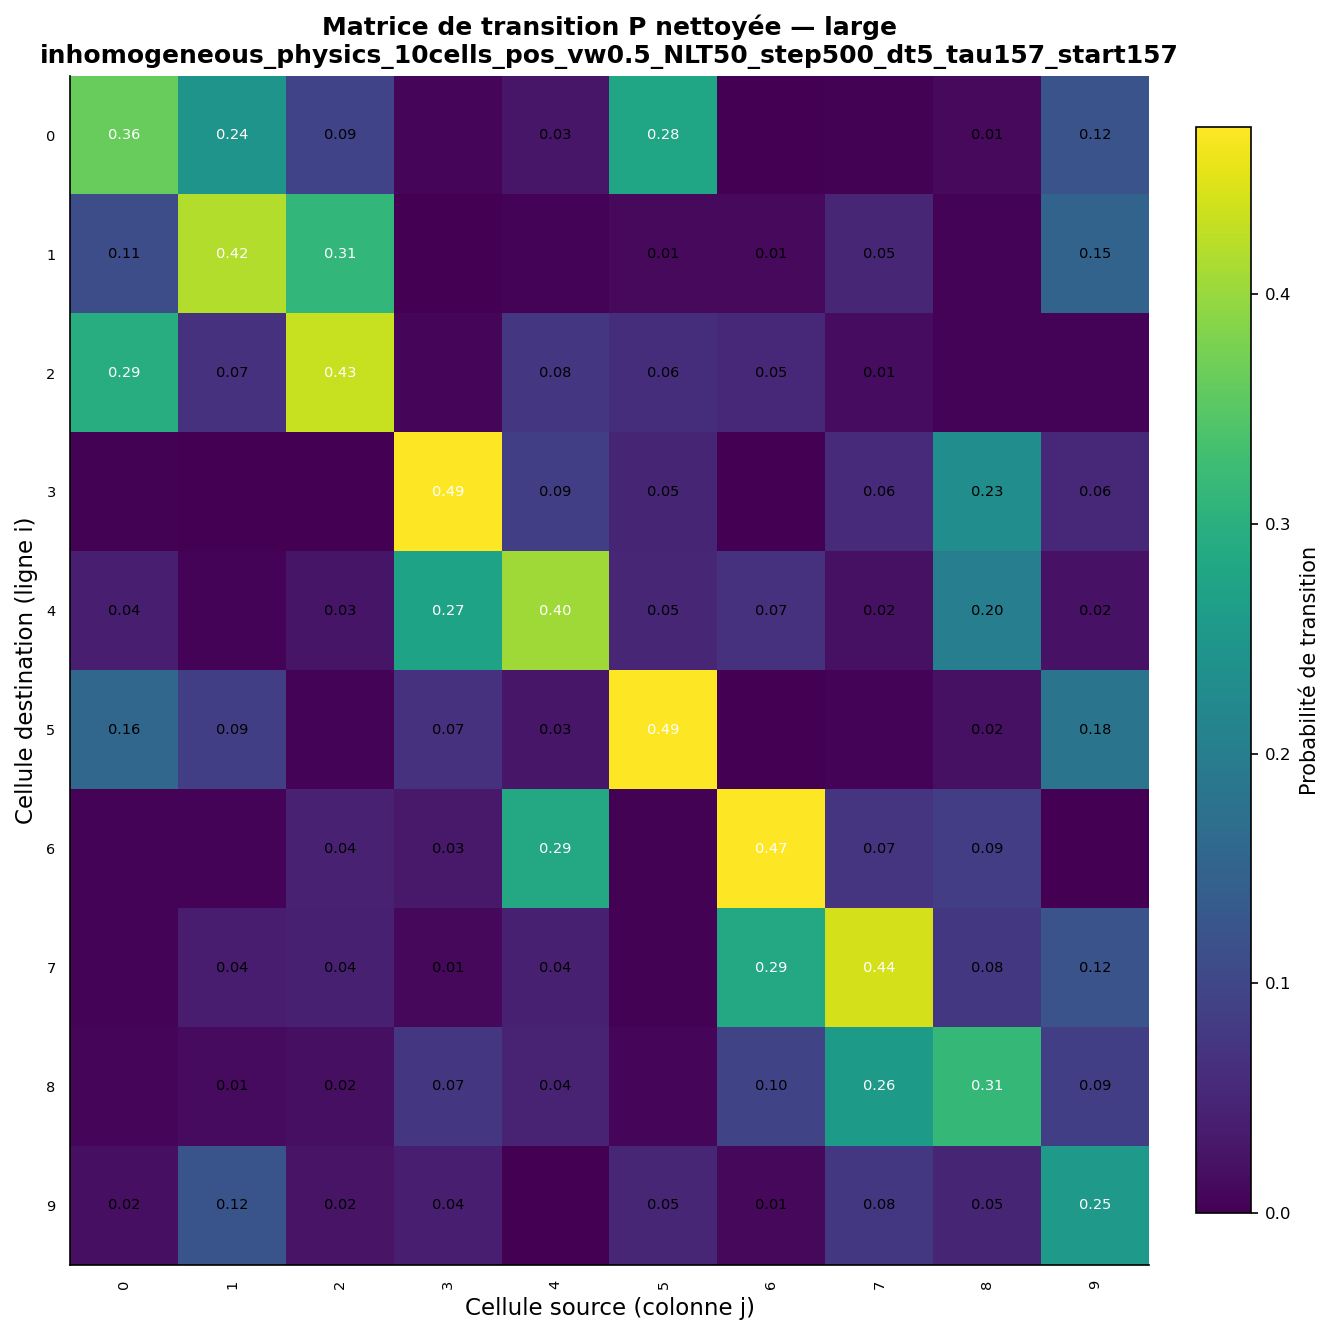
\includegraphics[width=\linewidth]{figures/matrice_physique_grandes.png}
    \subcaption*{(a) Grandes particules}
  \end{minipage}\hfill
  \begin{minipage}{0.48\textwidth}
    \centering
    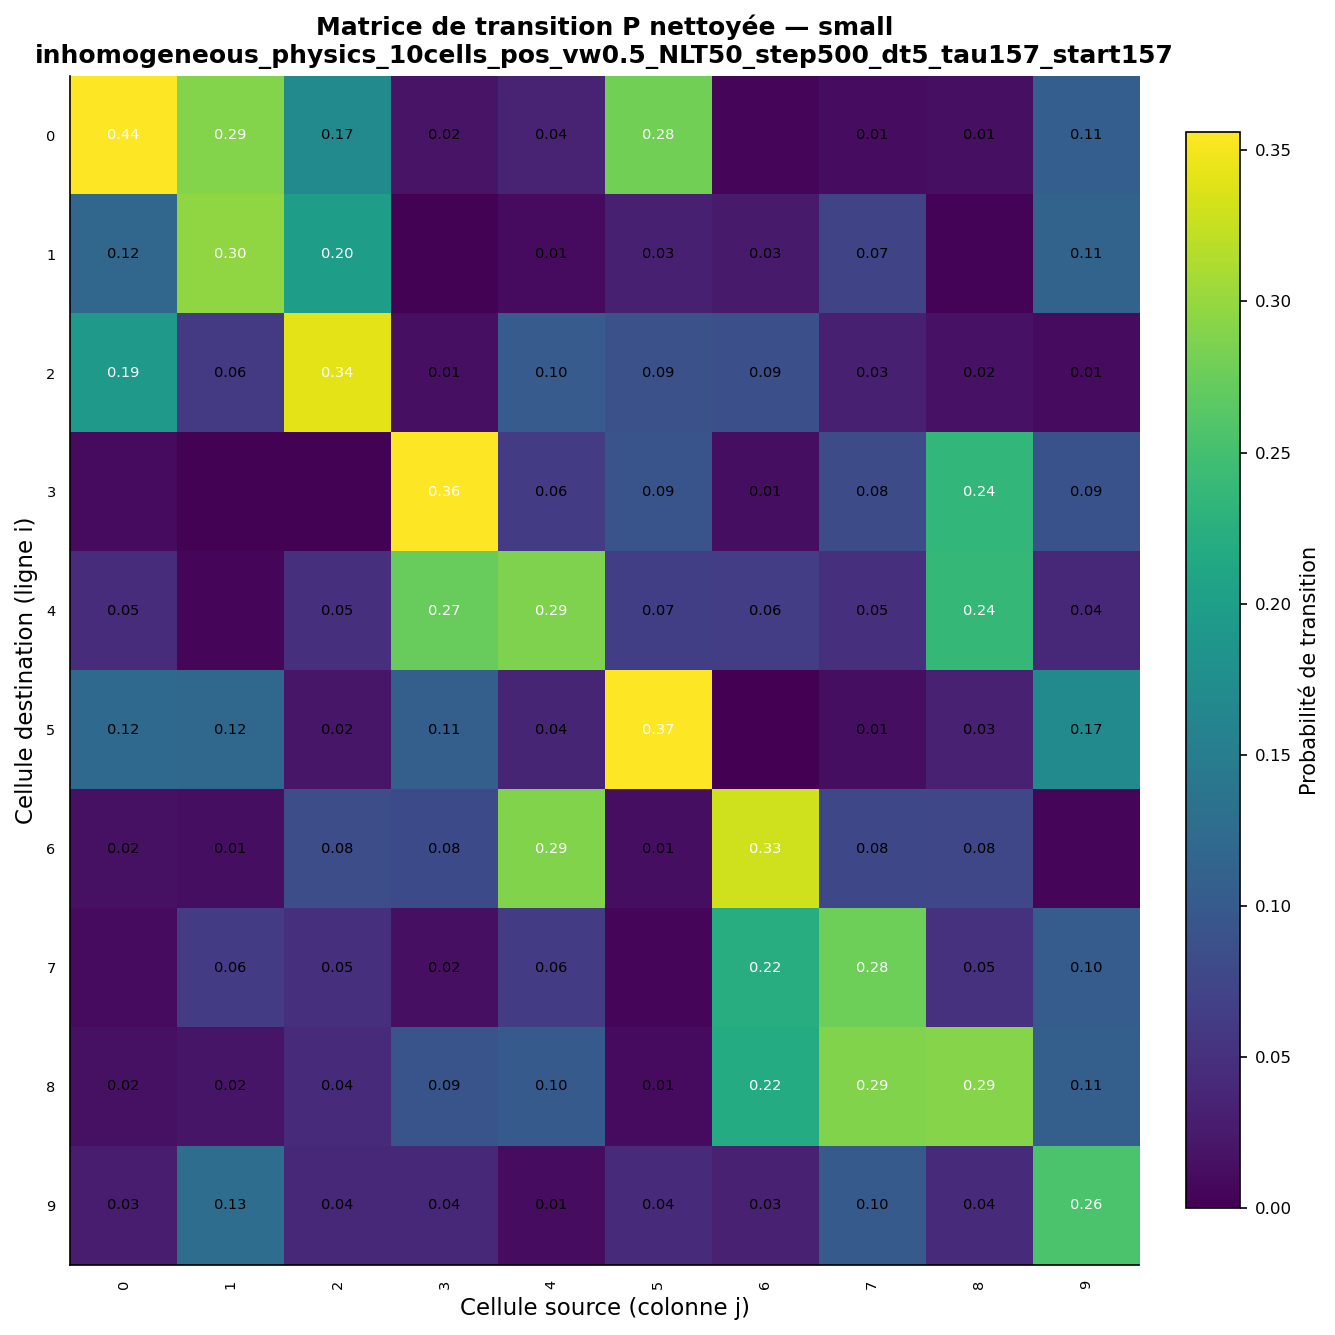
\includegraphics[width=\linewidth]{figures/matrice_physique_petites.png}
    \subcaption*{(b) Petites particules}
  \end{minipage}
  \caption{Matrices de transition (découpage physique) pour chaque espèce.}
  \label{fig:matrice_physique}
\end{figure}

Les chaînes homogènes fournissent une première estimation acceptable, mais les chaînes inhomogènes, en actualisant les probabilités à chaque intervalle, suivent plus fidèlement la trajectoire DEM (figure~\ref{fig:teneur_physique}).

\begin{figure}[H]
  \centering
  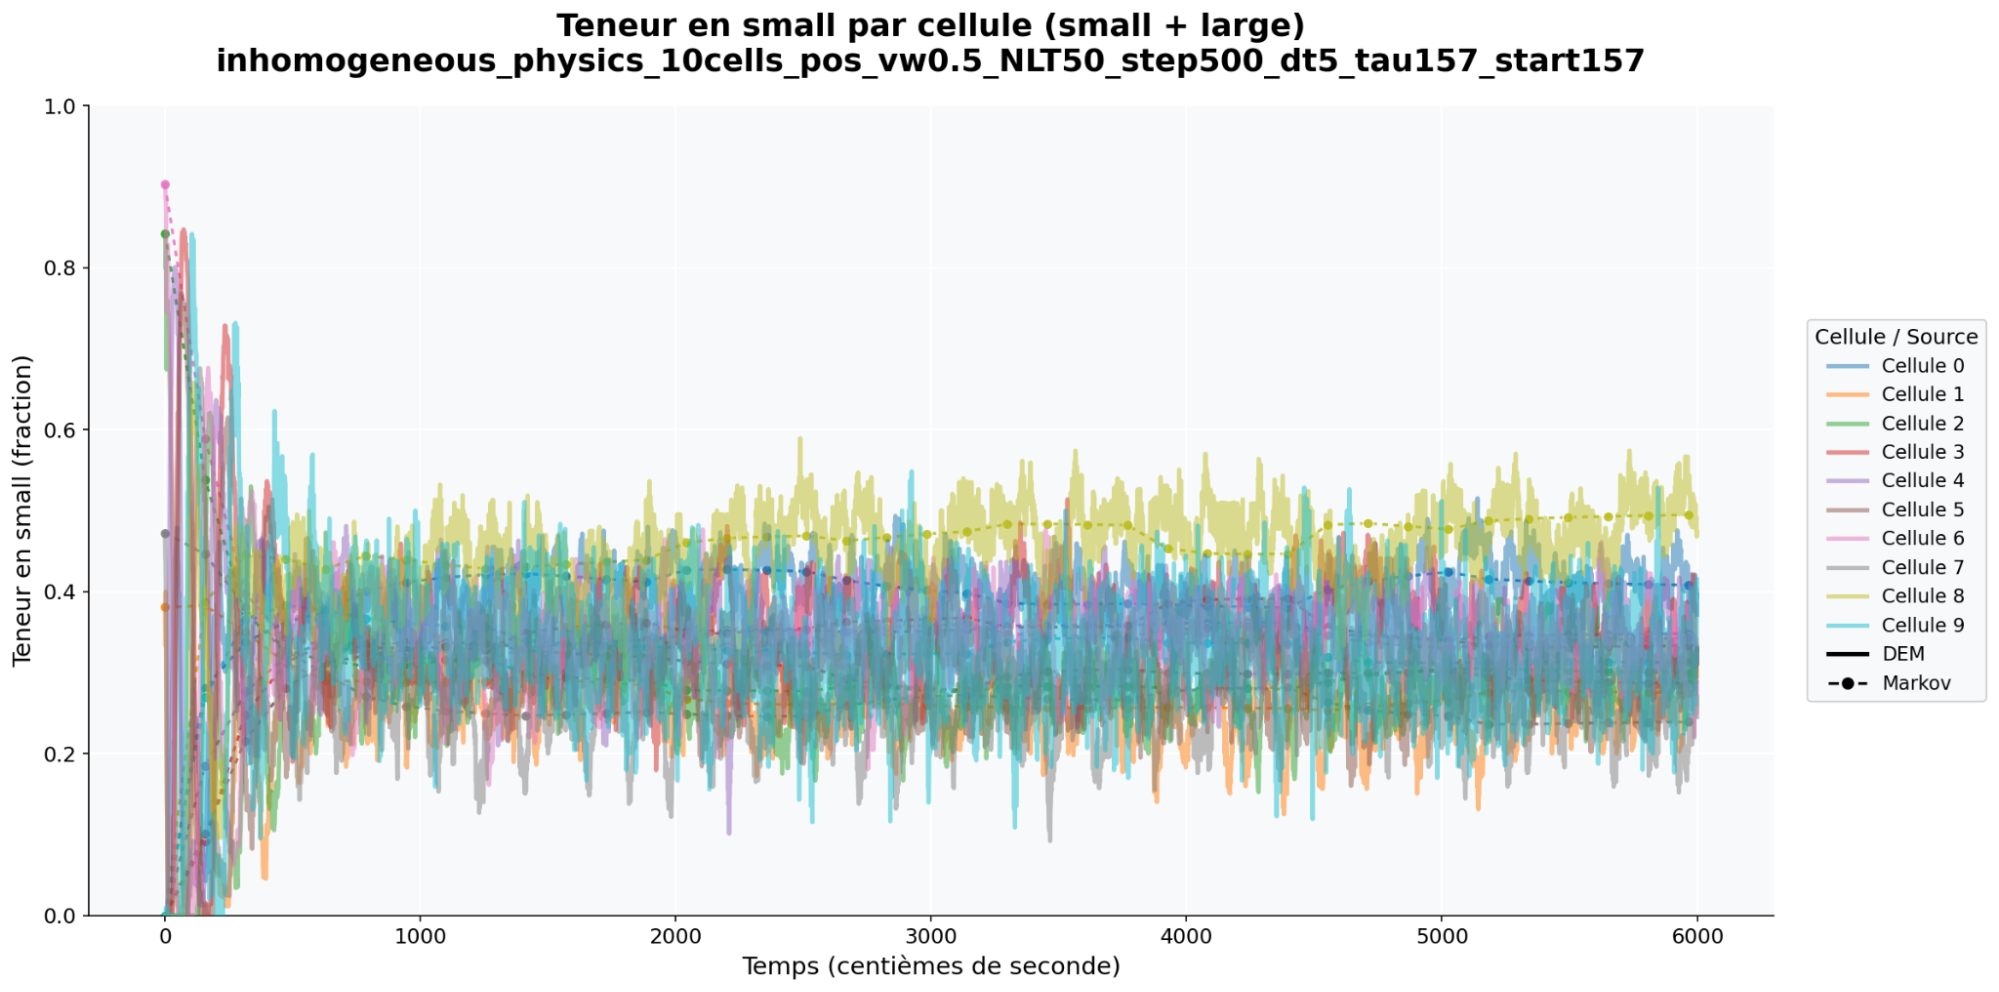
\includegraphics[width=0.85\textwidth]{figures/comparaison_dem_markov.png}
  \caption{Évolution de la teneur en petites particules : découpage physique, chaîne inhomogène.}
  \label{fig:teneur_physique}
\end{figure}

Le RSD calculé pour chaque type de chaîne (figure~\ref{fig:rsd_physique}) confirme cette hiérarchie : la chaîne inhomogène produit des valeurs sensiblement plus proches de la DEM que la chaîne homogène.

\begin{figure}[H]
  \centering
  \begin{minipage}{0.48\textwidth}
    \centering
    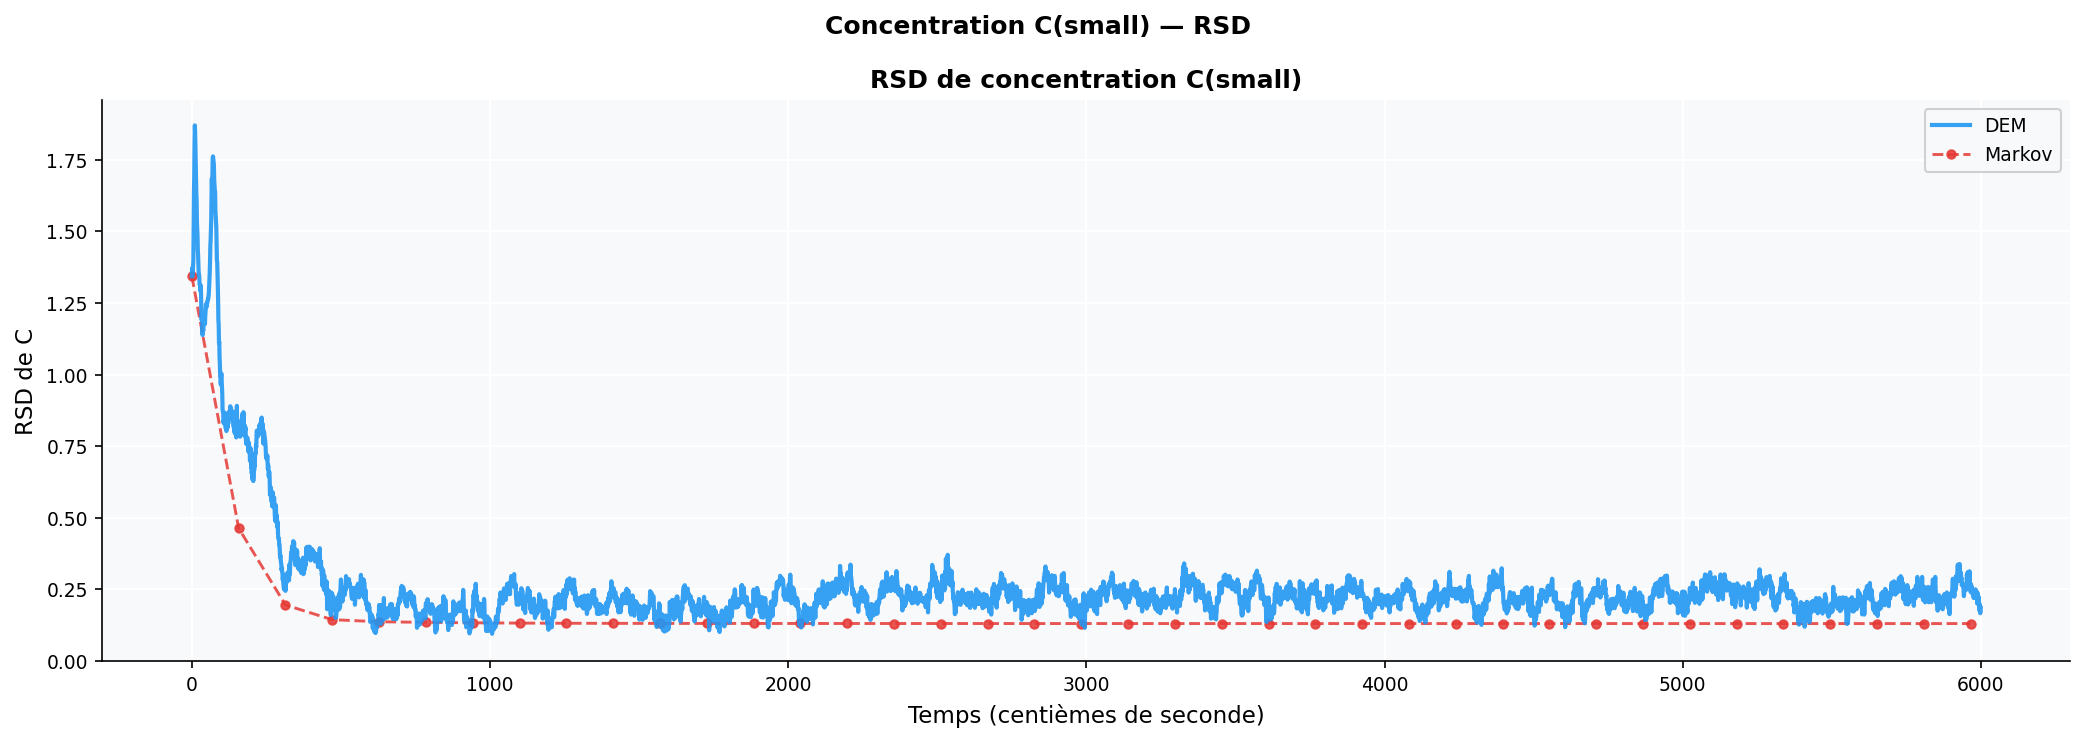
\includegraphics[width=\linewidth]{figures/rsd_physic.png}
    \subcaption*{(a) Chaîne homogène}
  \end{minipage}\hfill
  \begin{minipage}{0.48\textwidth}
    \centering
    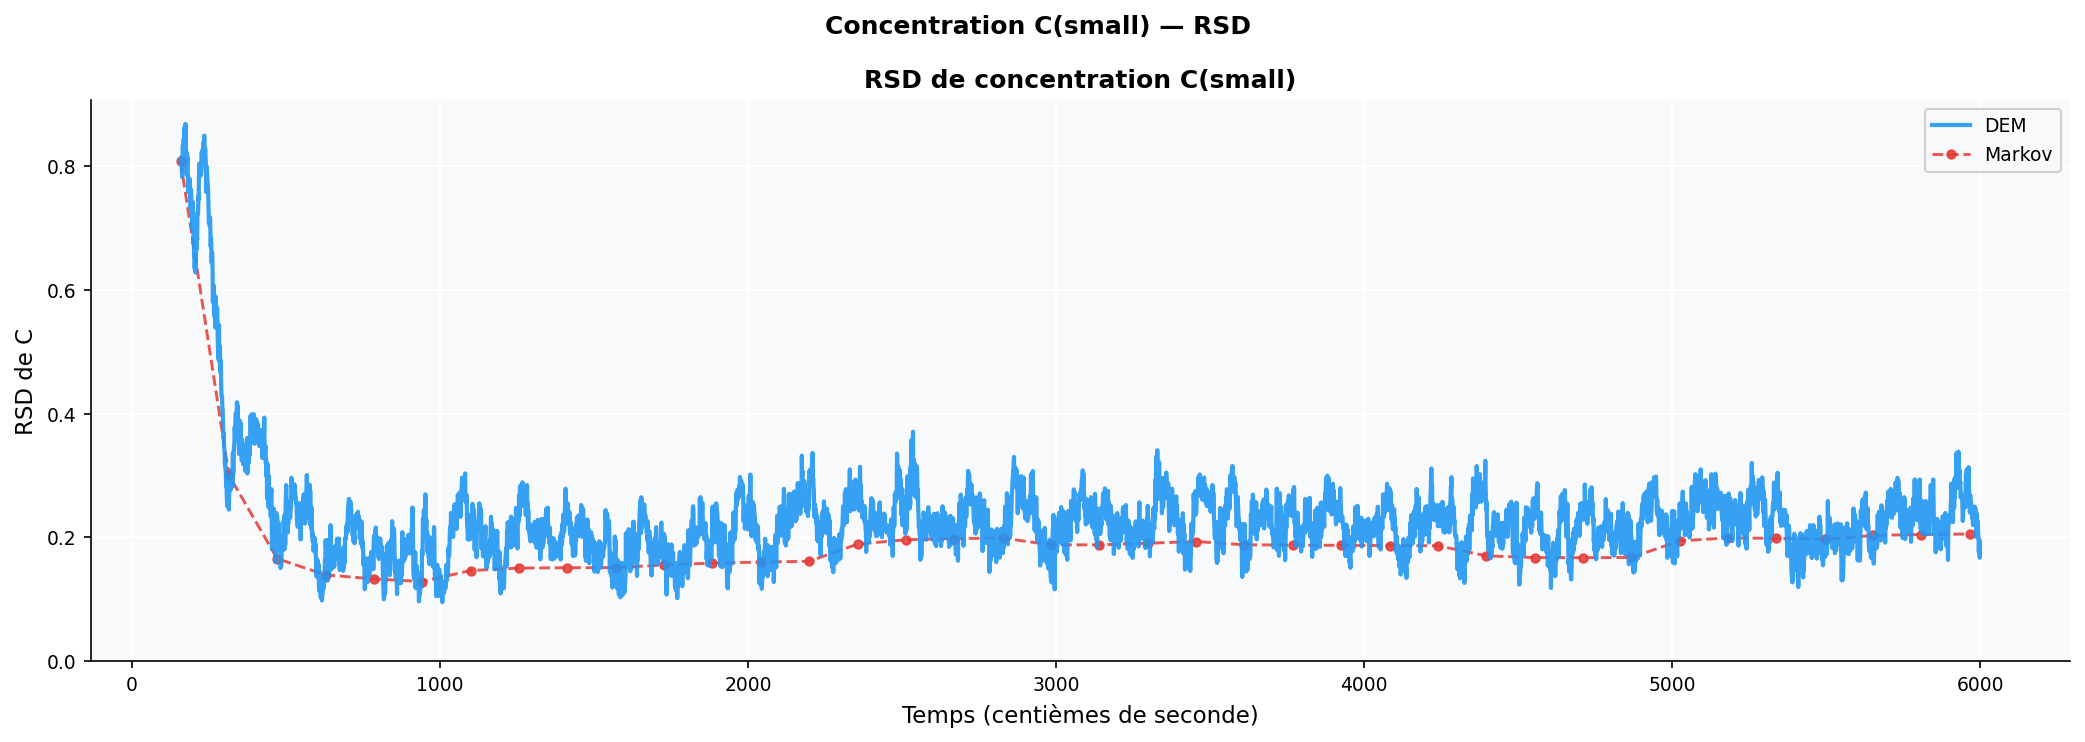
\includegraphics[width=\linewidth]{figures/rsd_physic_inhomogene.png}
    \subcaption*{(b) Chaîne inhomogène}
  \end{minipage}
  \caption{RSD de la concentration en petites particules : DEM vs.\ Markov homogène et inhomogène (découpage physique).}
  \label{fig:rsd_physique}
\end{figure}

\subsection{Influence du choix de la discrétisation}

Le tableau~\ref{tab:erreur_methodes} rassemble, pour les trois méthodes, l'écart temporel moyen $|\text{Markov}-\text{DEM}|$, l'écart absolu toutes cellules confondues et l'erreur RMS.

\begin{table}[H]
  \centering
  \caption{Erreur de prédiction markovienne par méthode de discrétisation et par espèce.}
  \label{tab:erreur_methodes}
  \begin{tabular}{@{}lcc@{}}
    \toprule
    Méthode & \multicolumn{1}{c}{Grandes particules} & \multicolumn{1}{c}{Petites particules} \\
    \midrule
    Cartésien &
    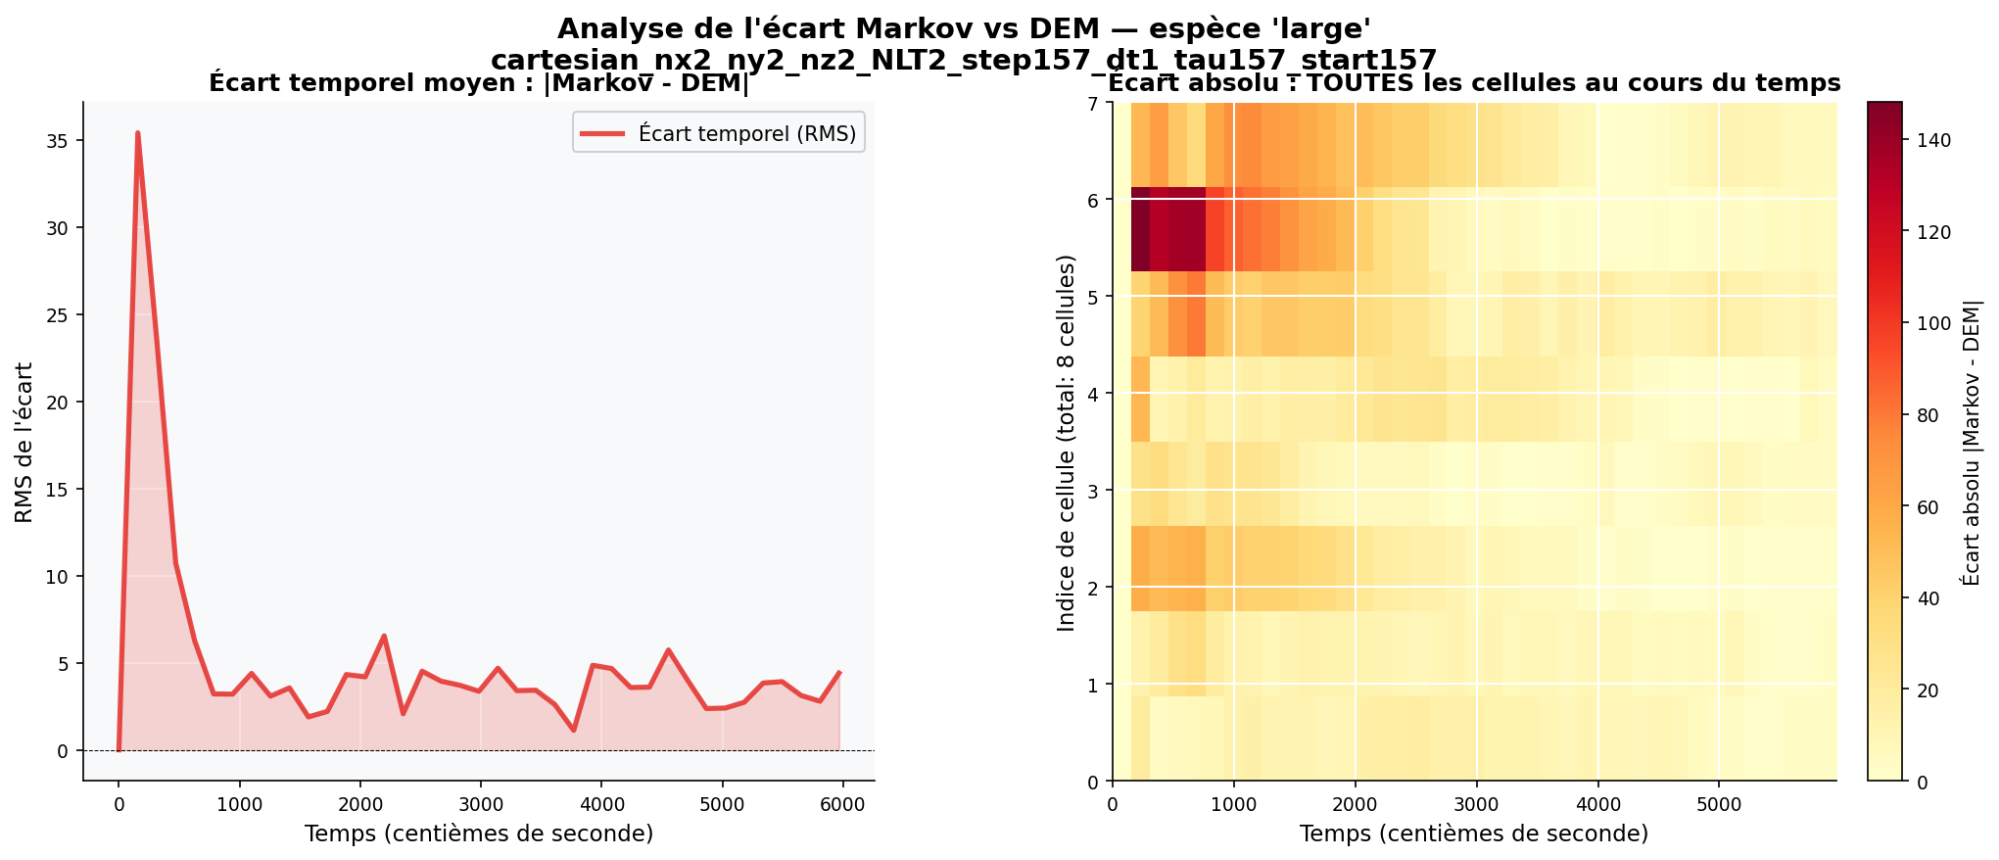
\includegraphics[width=0.42\textwidth]{figures/erreur_cartesien_grandes.png} &
    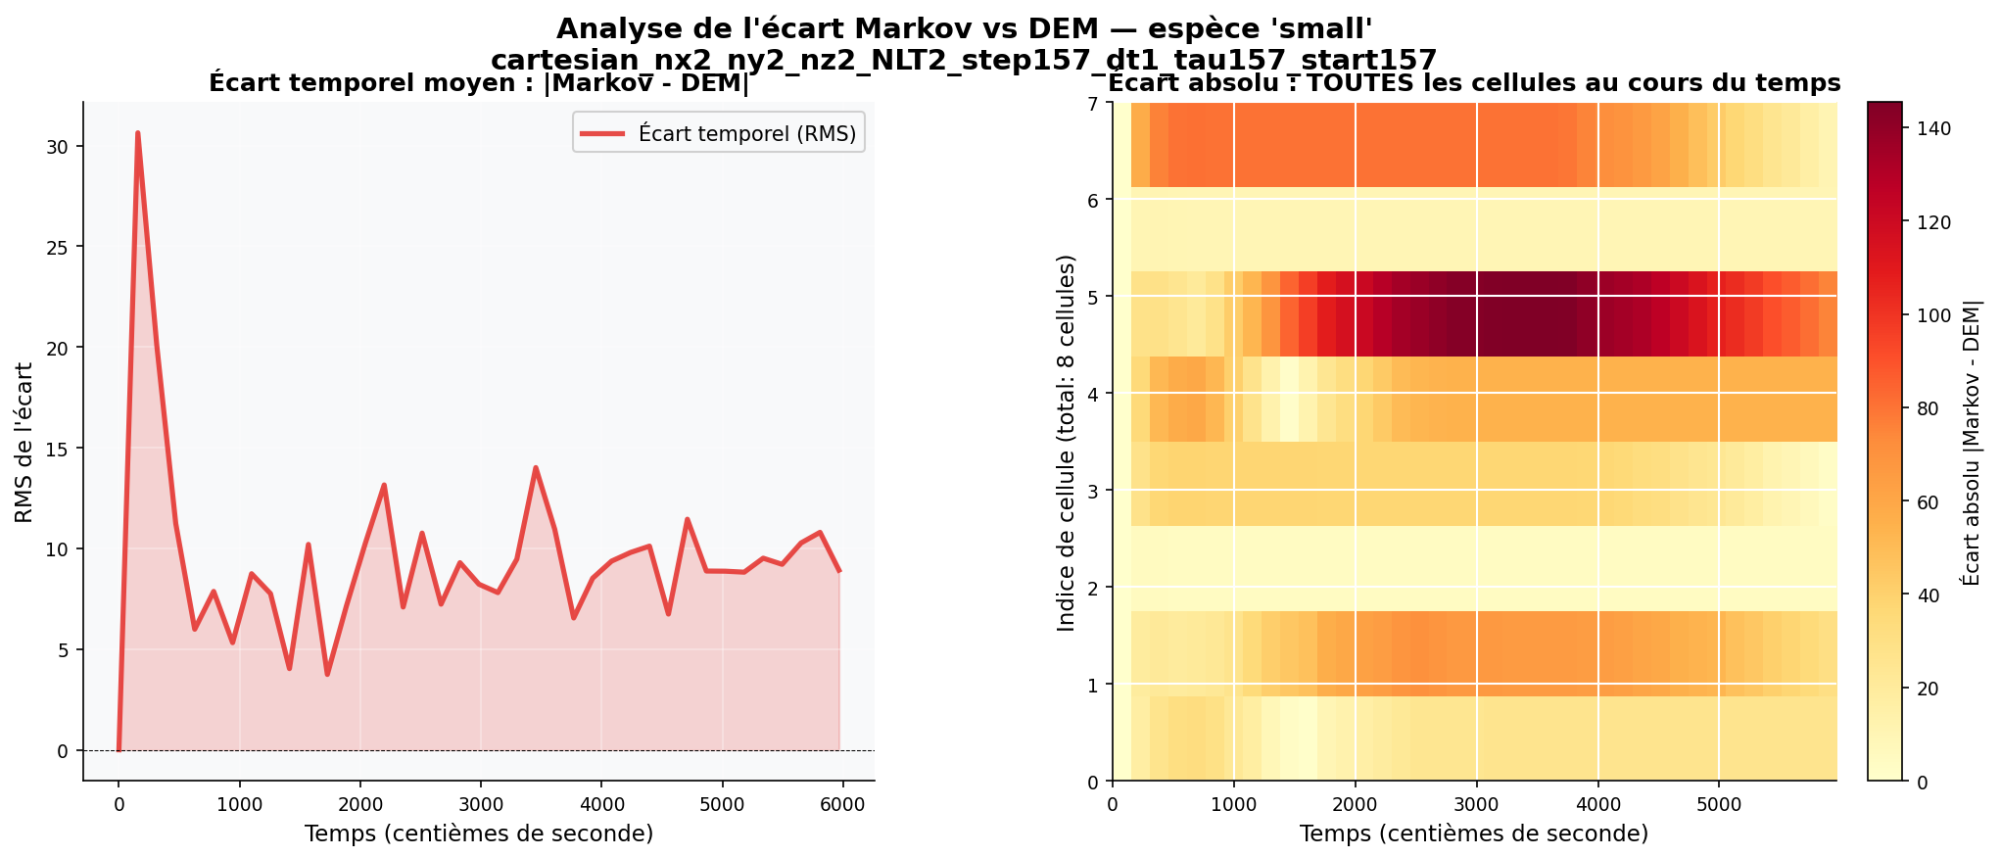
\includegraphics[width=0.42\textwidth]{figures/erreur_cartesien_petites.png} \\
    \addlinespace
    Voronoï &
    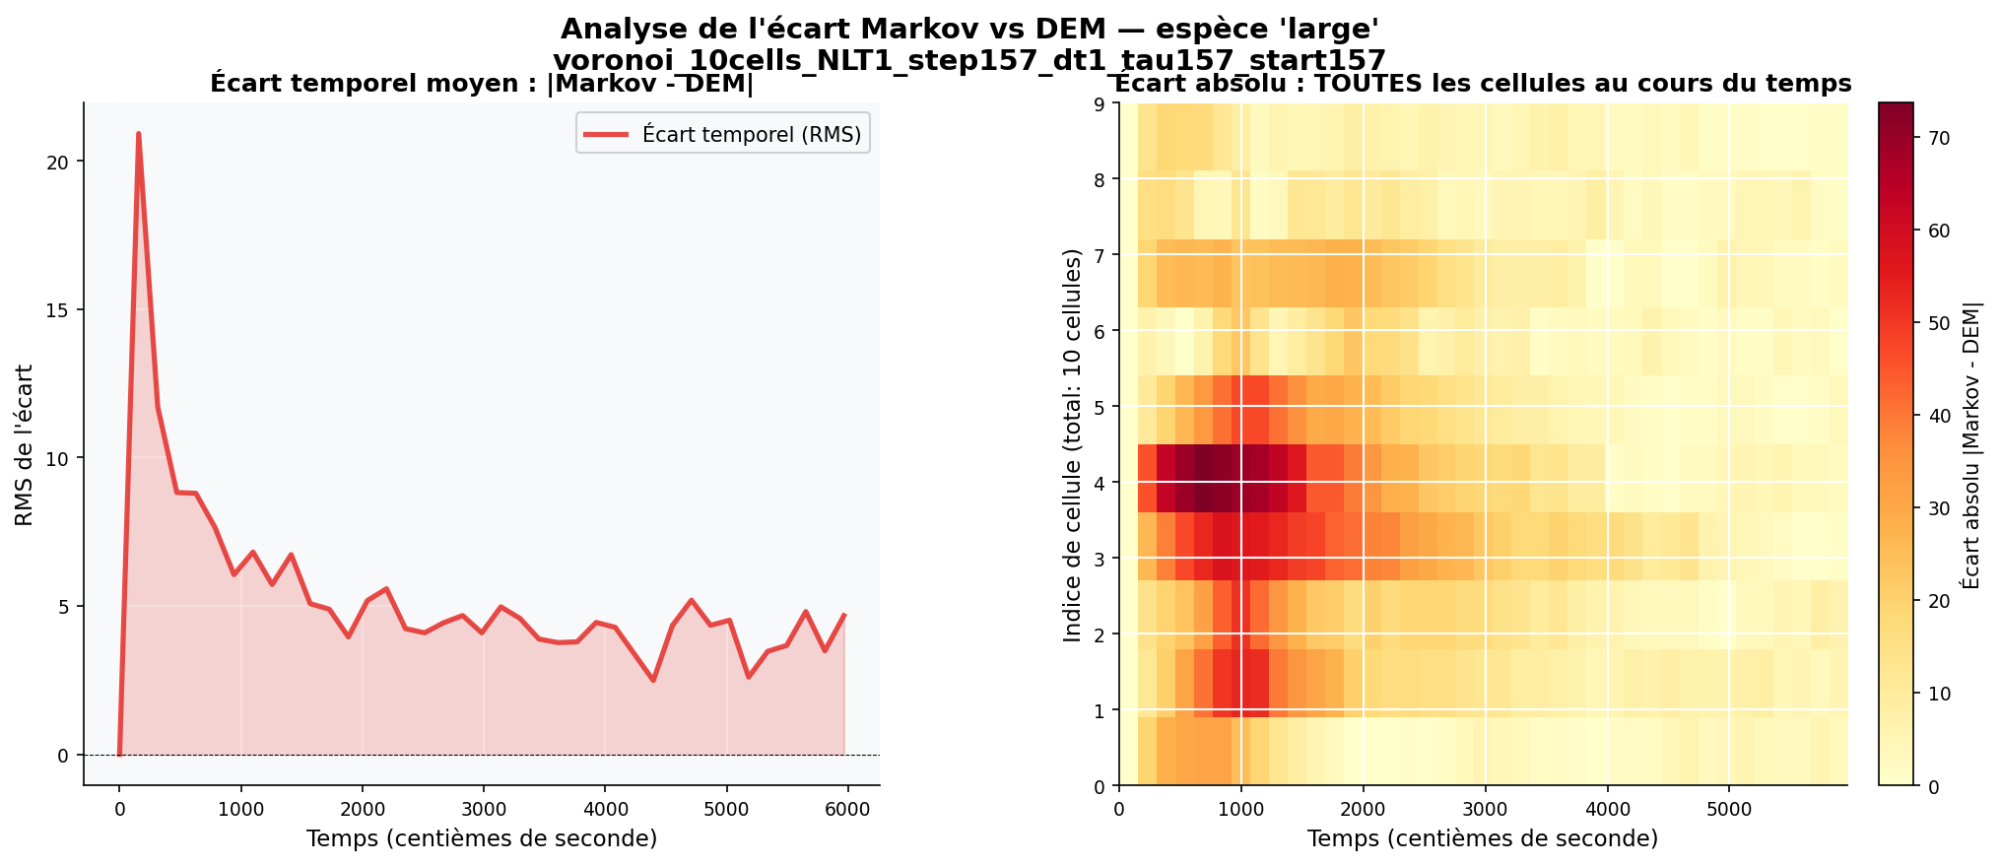
\includegraphics[width=0.42\textwidth]{figures/erreur_voronoi_grandes.png} &
    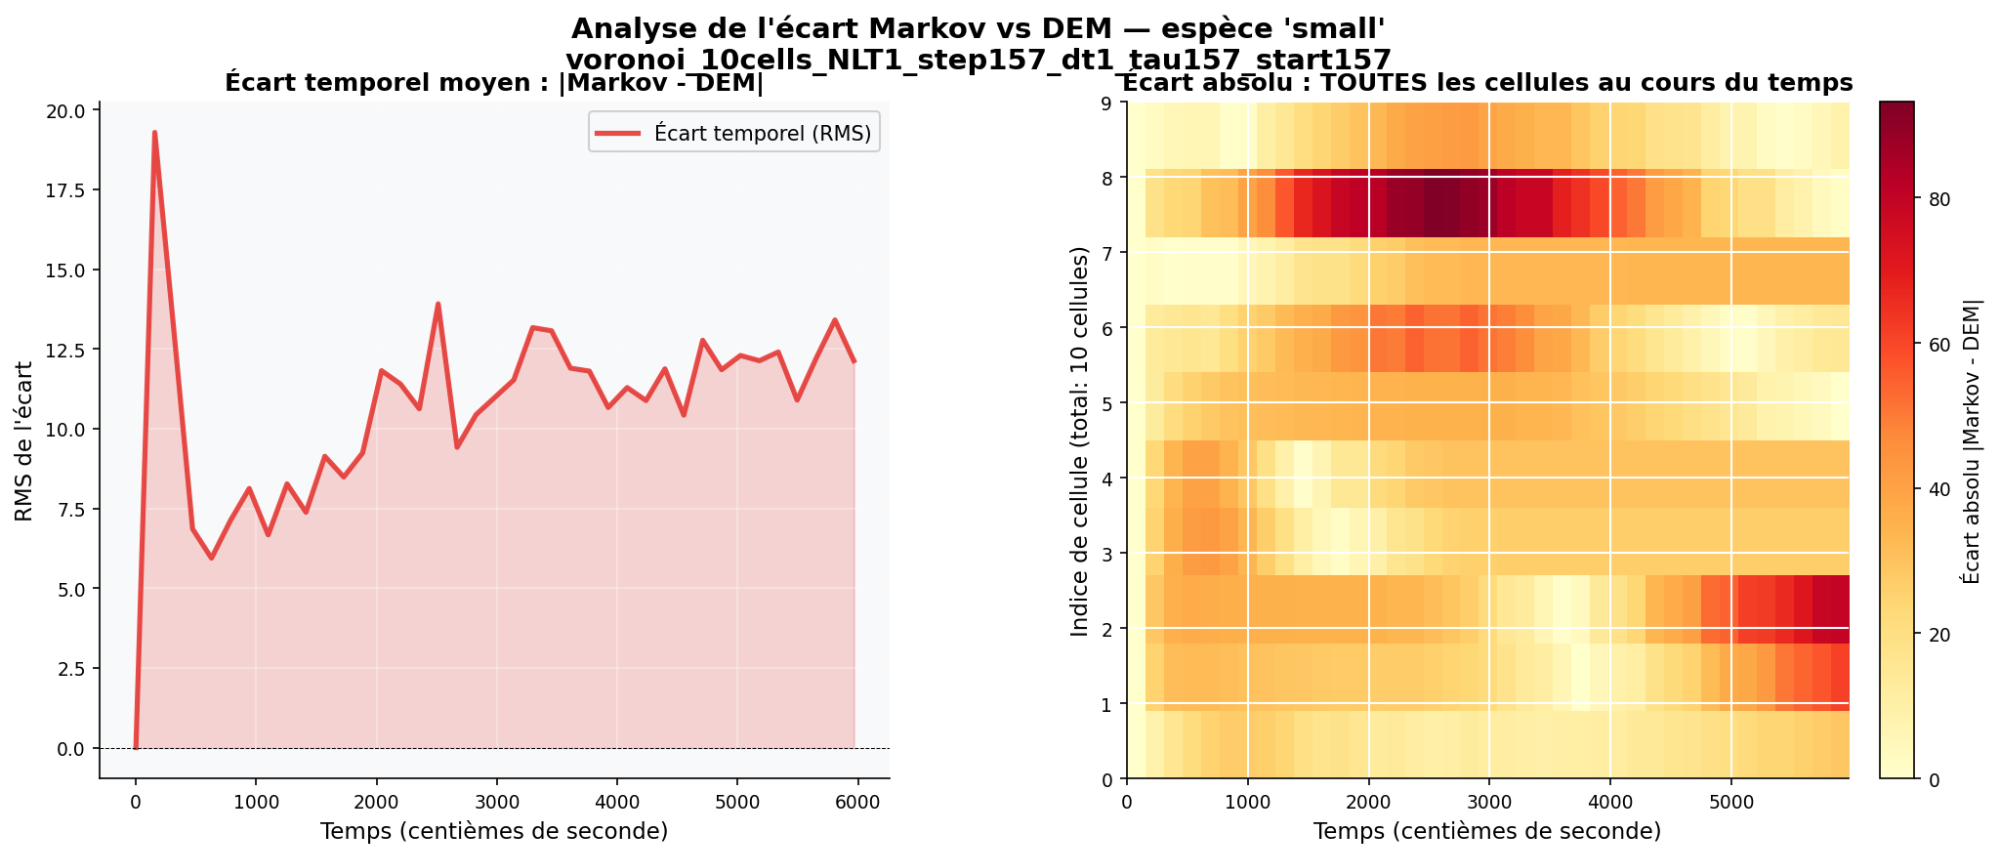
\includegraphics[width=0.42\textwidth]{figures/erreur_voronoi_petites.png} \\
    \addlinespace
    Physique &
    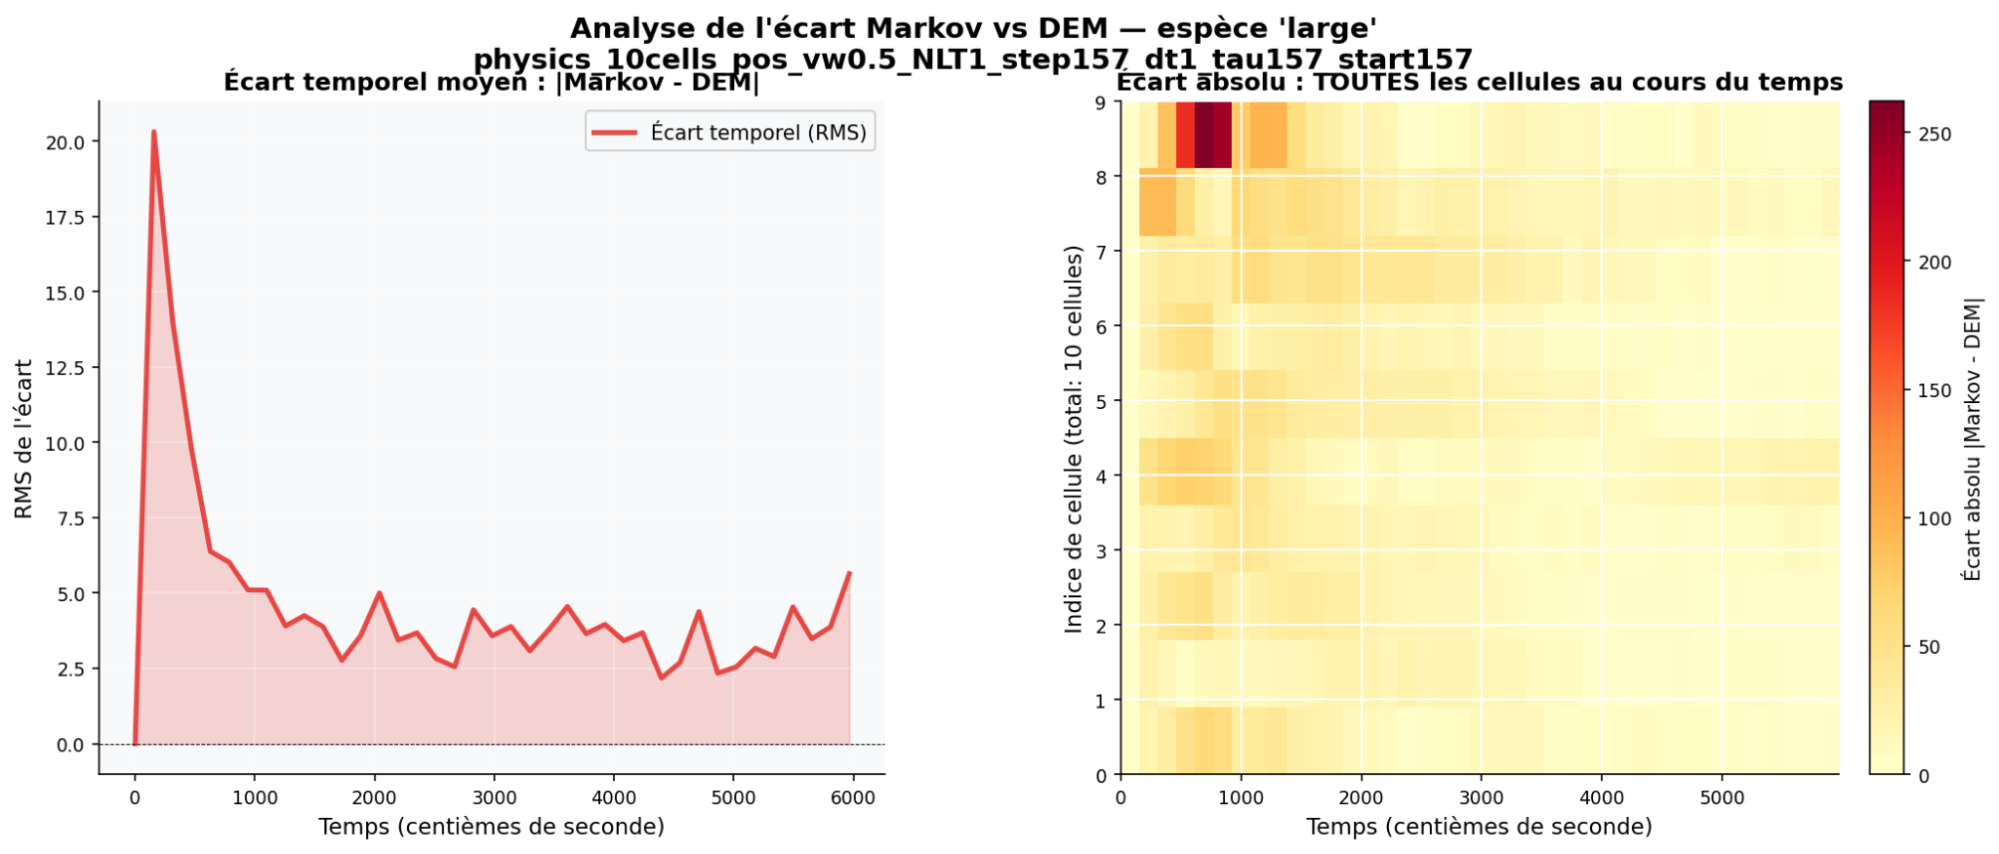
\includegraphics[width=0.42\textwidth]{figures/erreur_physique_grandes.png} &
    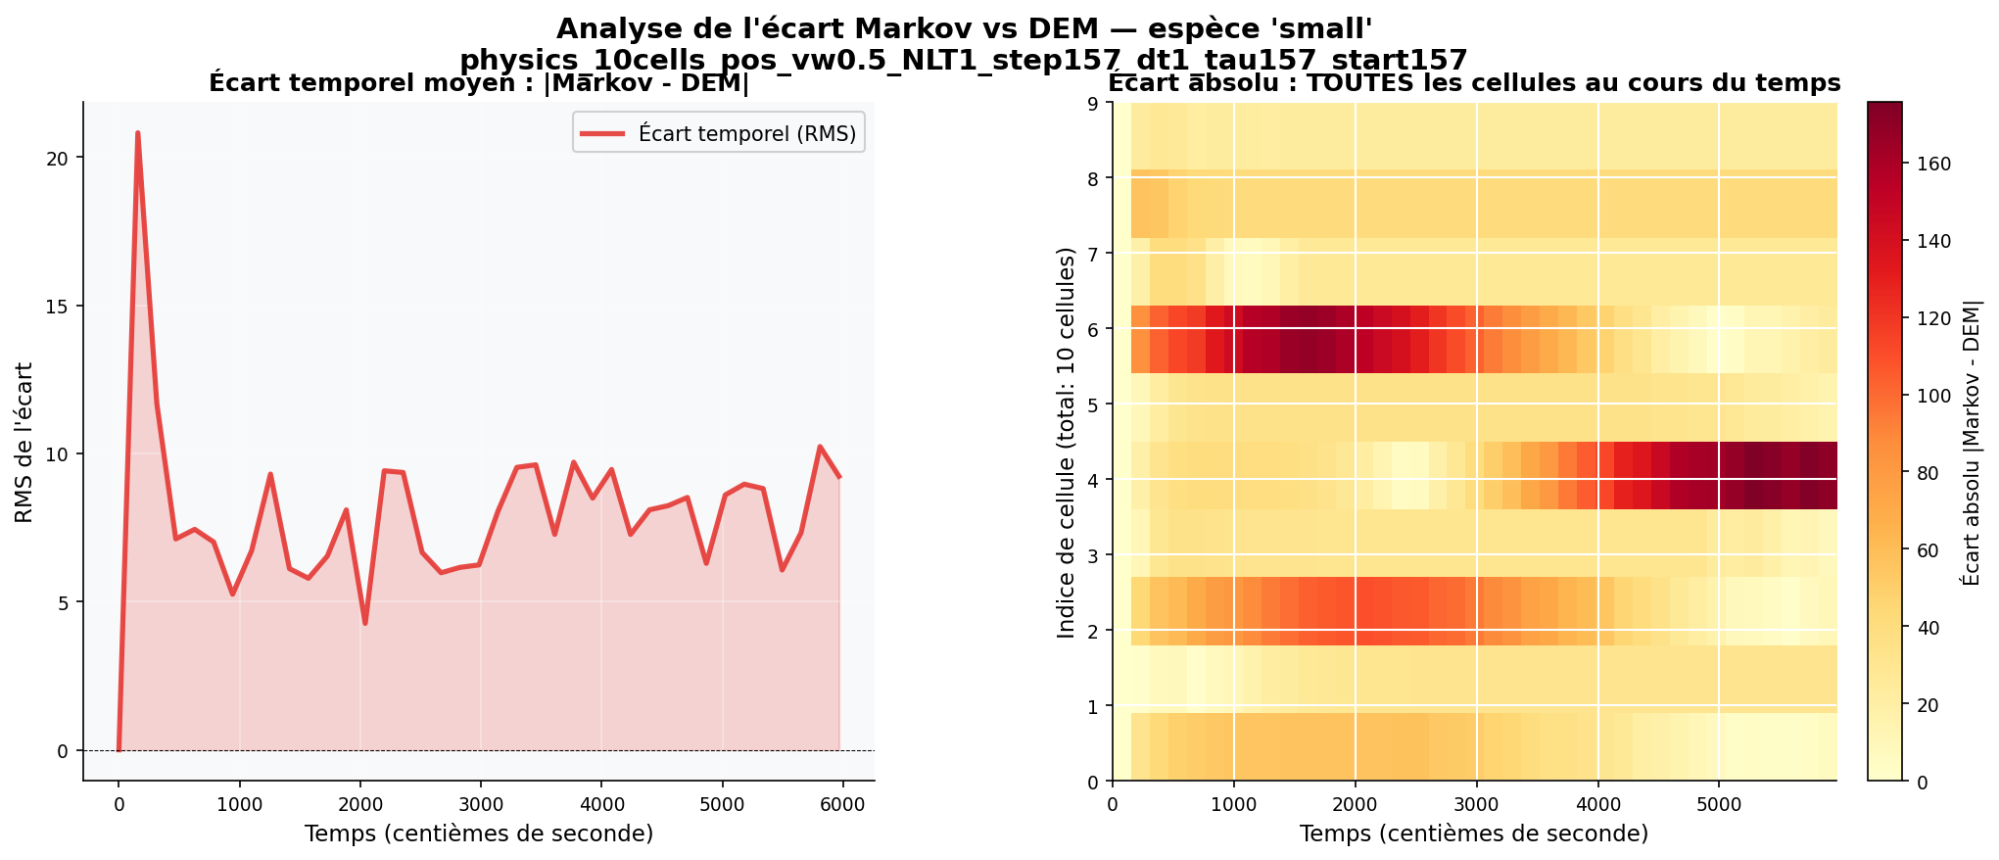
\includegraphics[width=0.42\textwidth]{figures/erreur_physique_petites.png} \\
    \bottomrule
  \end{tabular}
\end{table}

La comparaison des trois rangées révèle des différences substantielles tant en amplitude qu'en morphologie de l'erreur. Le modèle de Markov est donc fortement conditionné par la manière dont l'espace est partitionné : la robustesse de la prédiction ne dépend pas uniquement de la physique du mélange, mais aussi --- et peut-être surtout --- du choix de maillage.

% ============================================================
% DISCUSSION
% ============================================================
\section{Discussion}

Trois enseignements principaux se dégagent de l'ensemble de ces résultats.

\paragraph{Dualité de comportement entre espèces.} Les matrices de transition, quelle que soit la méthode de maillage, montrent systématiquement que les grandes particules restent plus longtemps dans leur cellule d'origine tandis que les petites se redistribuent plus rapidement. Cette asymétrie, cohérente avec les mécanismes de percolation et de convection dans un tambour tournant, justifie pleinement la construction de matrices séparées.

\paragraph{Rôle déterminant de la discrétisation.} Un maillage purement géométrique, bien que simple à mettre en œuvre, peut produire des cellules peu représentatives de la distribution effective des grains. Les approches statistiques --- Voronoï, physique --- adaptent les partitions à la configuration réelle du lit et réduisent l'erreur de prédiction, comme en témoigne le tableau~\ref{tab:erreur_methodes}.

\paragraph{Pertinence de la variable d'état.} Le comptage par cellule décrit l'occupation globale mais masque la ségrégation. La teneur locale en petites particules, en revanche, fait apparaître des hétérogénéités marquées (cellules 9 et 4, par exemple) et offre un indicateur directement relié au phénomène physique étudié.

Enfin, les chaînes inhomogènes se révèlent indispensables dès que l'on souhaite capturer les phases transitoires ou les variations temporelles des probabilités de transition, là où l'hypothèse stationnaire d'une chaîne homogène atteint ses limites. Le piégeage des particules dans les zones passives, visible à travers les fortes probabilités diagonales, souligne par ailleurs la nécessité d'un maillage capable de résoudre la coexistence entre zone active de surface et zone quasi-statique en profondeur.

% ============================================================
% CONCLUSION ET PERSPECTIVES
% ============================================================
\section{Conclusion et perspectives}
\label{sec:conclusion}

Ce mémoire a proposé et évalué une modélisation stochastique par chaînes de Markov pour reproduire la ségrégation de particules bidisperses dans un tambour tournant, à partir de données DEM de référence. Les principaux apports sont les suivants :

\begin{itemize}
  \item La construction de matrices de transition distinctes par espèce met en évidence des dynamiques contrastées entre petites et grandes particules.
  \item Le choix de la discrétisation spatiale conditionne fortement la fidélité du modèle : les maillages statistiques (Voronoï, physique) surpassent les maillages géométriques en termes d'erreur de prédiction.
  \item Un vecteur d'état fondé sur la teneur locale en petites particules discrimine la ségrégation bien mieux qu'un simple comptage.
  \item Les chaînes inhomogènes, en actualisant les probabilités à chaque pas, suivent plus fidèlement l'évolution DEM que les chaînes homogènes, en particulier durant les régimes transitoires.
\end{itemize}

Plusieurs axes de prolongement se dessinent. Il serait pertinent de mener une étude paramétrique systématique --- nombre de cellules, pas de temps markovien, durée d'apprentissage --- afin de quantifier la sensibilité du modèle à ces réglages. L'extension à des configurations industrielles impliquant plusieurs millions de grains permettrait d'évaluer le compromis entre précision et coût computationnel. Enfin, l'intégration d'indicateurs de corrélation spatiale ou de fonctions de distribution radiale viendrait compléter le RSD pour une caractérisation plus fine de la structure du mélange.

% ============================================================
% BIBLIOGRAPHIE
% ============================================================
\cleardoublepage
\phantomsection
\addcontentsline{toc}{section}{Références bibliographiques}
\nocite{mellmann2001,morrison2016}
\printbibliography[
  heading=bibliographie,
  title={Références bibliographiques}
]

\end{document}